\pdfoutput=1
\documentclass[12pt]{amsart}
\usepackage[margin=20truemm]{geometry}
\usepackage[backend=biber, style=alphabetic]{biblatex}
\ExecuteBibliographyOptions{
    sorting=nyt,
    sortcites=false,
    date=year,
    urldate=iso,
    seconds=true,
    maxnames=8,minnames=3,
    maxalphanames=4,minalphanames=3,
    maxbibnames=99,
    giveninits=true,
    isbn=false,
    url=true,
    doi=false,
    eprint=true
}

\addbibresource{../bib/half-spherical-twist.bib}

\DeclareSourcemap{
  \maps[datatype=bibtex]{
    \map{
      \step[fieldsource=url, 
            match=\regexp{https?://(dx\.)?doi(-|\.)org}, 
            final]
      \step[fieldset=url, null]
      \step[fieldset=urldate, null]
    }
  }
}


\AtEveryBibitem{%
    \ifentrytype{book}{\clearfield{pages}}{}%
}

\DeclareFieldFormat{pages}{#1}
\renewbibmacro{in:}{}
\renewcommand{\multicitedelim}{\addcomma\space}

\DeclareFieldFormat[article]{number}{\bibstring{number}~#1}
\renewbibmacro*{journal+issuetitle}{%
	\usebibmacro{journal}%
	\setunit*{\addspace}%
	\iffieldundef{series}
	{}
	{\newunit
		\printfield{series}%
		\setunit{\addspace}}%
	\printfield{volume}%
	\setunit{\addspace}%
	\usebibmacro{issue+date}%
	\setunit{\addcolon\space}%
	\usebibmacro{issue}%
	\setunit{\addcomma\space}%
	\printfield{number}%
	\setunit{\addcomma\space}%
	\printfield{eid}%
	\newunit
}

\DeclareFieldFormat[article, inproceedings]{title}{#1}

%% packages
\usepackage[svgnames]{xcolor}
\usepackage{mathtools}
\usepackage{tikz-cd}
\usepackage{amsmath, amssymb, amsthm}
\usepackage{here}
\usetikzlibrary{intersections, patterns, snakes}


\numberwithin{equation}{section}
\mathtoolsset{showonlyrefs=true}
\renewcommand{\theenumi}{\arabic{enumi}}

%% Theorems
\theoremstyle{plain}

\newtheorem{theorem}{Theorem}[section]
\newtheorem{conjecture}[theorem]{Conjecture}
\newtheorem{lemma}[theorem]{Lemma}
\newtheorem{proposition}[theorem]{Proposition}
\newtheorem{corollary}[theorem]{Corollary}

\theoremstyle{definition}
\newtheorem{definition}[theorem]{Definition}
\newtheorem{example}[theorem]{Example}
\newtheorem{remark}[theorem]{Remark}

%% Some operators
\DeclareMathOperator{\Hom}{\mathrm{Hom}}
\DeclareMathOperator{\Tor}{\mathrm{Tor}}
\DeclareMathOperator{\CHom}{\mathcal{H}\!\mathit{om}}
\DeclareMathOperator{\CTor}{\mathcal{T}\!\mathit{or}}
\DeclareMathOperator{\Auteq}{\mathrm{Auteq}}
\DeclareMathOperator{\Cone}{\mathrm{Cone}}
\DeclareMathOperator{\ev}{\mathrm{ev}}
\DeclareMathOperator{\id}{\mathrm{id}}
\DeclareMathOperator{\depth}{\mathrm{depth}}
\DeclareMathOperator{\Pic}{\mathrm{Pic}}
\DeclareMathOperator{\MCG}{\mathrm{MCG}}
\DeclareMathOperator{\PMCG}{\mathrm{PMCG}}
\DeclareMathOperator{\RHom}{\mathrm{RHom}}
\DeclareMathOperator{\Ker}{\mathrm{Ker}}
\DeclareMathOperator{\Image}{\mathrm{Im}}
\DeclareMathOperator{\Aut}{\mathrm{Aut}}
\DeclareMathOperator{\Inn}{\mathrm{Inn}}
\DeclareMathOperator{\Out}{\mathrm{Out}}
\DeclareMathOperator{\Supp}{\mathrm{Supp}}
\DeclareMathOperator{\SL}{\mathrm{SL}}
\DeclareMathOperator{\Spec}{\mathrm{Spec}}
\DeclareMathOperator{\Perf}{\mathrm{Perf}}
\DeclareMathOperator{\NS}{\mathrm{NS}}
\DeclareMathOperator{\Ext}{\mathrm{Ext}}
\DeclareMathOperator{\Hilb}{\mathrm{Hilb}}
\DeclareMathOperator{\FM}{\mathrm{FM}}
\DeclareMathOperator{\res}{\mathrm{res}}

\newcommand{\nc}{\newcommand}

%% Calligraphic letters
\nc{\cE}{{\mathcal{E}}}
\nc{\cF}{{\mathcal{F}}}
\nc{\cG}{{\mathcal{G}}}
\nc{\cH}{{\mathcal{H}}}

\nc{\cO}{{\mathcal{O}}}
\nc{\cP}{{\mathcal{P}}}
\nc{\cQ}{{\mathcal{Q}}}

\nc{\cU}{{\mathcal{U}}}
\nc{\cW}{{\mathcal{W}}}

%% Blackboard letters
\nc{\bA}{{\mathbb{A}}}
\nc{\bC}{{\mathbb{C}}}
\nc{\bP}{{\mathbb{P}}}
\nc{\bQ}{{\mathbb{Q}}}
\nc{\bZ}{{\mathbb{Z}}}



\makeatletter
\newcommand*{\rom}[1]{\expandafter\@slowromancap\romannumeral #1@}
\makeatother




% hyperref 
\usepackage[
    colorlinks=true,
    citecolor=MediumBlue,
    urlcolor=MediumBlue,
    linkcolor=MediumBlue,
    breaklinks=true,
]{hyperref}



\title[Half-spherical twists]{
    Half-spherical twists on derived categories\\ of coherent sheaves
    }
\author[H.~Arai]{Hayato Arai}
\address{
Graduate School of Mathematical Sciences,
The University of Tokyo,
3-8-1 Komaba,
Meguro-ku,
Tokyo,
153-8914,
Japan.
}
\email{hayato@ms.u-tokyo.ac.jp}
\begin{document}
\begin{abstract}
    For a flat morphism $\pi \colon X \to T$ between smooth quasi-projective varieties and its fiber $X_0$,
    we prove that spherical objects on $D^b(X)$ pushed-forward from $D^b(X_0)$ induce autoequivalences of $D^b(X_0)$ itself.
    Our construction provides new derived symmetries for some singular varieties, which include singular fibers of elliptic surfaces (commonly referred to as Kodaira fibers) and type \rom{3} degenerations of K3 surfaces.
    In the case of Kodaira fibers of type $\rom{1}_n$, we also show the induced autoequivalences of $D^b(X_0)$
    correspond to the \emph{half twists} on the $n$-punctured $2$-torus via homological mirror symmetry.
    As an application, we describe the autoequivalence groups of elliptic surfaces
    in terms of mapping class groups of punctured tori.
\end{abstract}
\maketitle

\section{Introduction}
Let $X$ be a complex projective variety and $D^b(X)$ be the bounded derived category of coherent sheaves on $X$.
The group consisting of the isomorphism classes of $\bC$-linear exact autoequivalences of $D^b(X)$
is denoted by $\Auteq{D^b(X)}$.
There are always three fundamental types of autoequivalences for any $X$: pulling back by automorphisms of $X$, tensoring line bundles, and the shift functor.
The subgroup generated by these autoequivalences
\begin{equation}
    \Aut{X} \ltimes \Pic{X} \times \bZ[1] \subset \Auteq{D^b(X)}
\end{equation}
is denoted by $A(X)$ and its elements
are called \emph{standard autoequivalences}.

Bondal and Orlov \cite{MR1818984} showed that $A(X) = \Auteq{D^b(X)}$ holds when $X$ is smooth projective, and either the canonical bundle $\omega_X$ or its dual is ample.
The simplest example that does not satisfy this condition is an elliptic curve.
In that case, we have an exact sequence
\begin{equation}\label{eq:autoequivalence-of-elliptic-curve}
    1 \to \Aut{X} \ltimes \Pic^{0}(X)\times \bZ[2] \to \Auteq{D^b(X)} \xrightarrow{\theta} \SL(2, \bZ) \to 1.
\end{equation}
This is a special case of Orlov's result \cite{MR1921811} for abelian varieties,
which goes back to the work of Mukai \cite{MR607081}
where non-trivial (auto-)equivalences of derived categories of abelian varieties were discovered.
The group homomorphism $\theta$ is given by the action on the Grothendieck group $K(X) \cong \bZ^2$. and one has $A(X) \subsetneq \Auteq{D^b(X)}$ by computing the image $\theta(A(X))$.
To construct non-standard autoequivalences explicitly,
the notion of \emph{twist functors along spherical objects},
or \emph{spherical twists} for short,
introduced by Seidel and Thomas \cite{MR1831820}, is useful.
For example, the twist $T_{\cO_X}$ along the structure sheaf $\cO_X$ is not standard when $X$ is an elliptic curve.

There are several other varieties for which the autoequivalence groups are (partially) determined.
They include toric surfaces \cite{MR3162236}, $K3$ surfaces \cite{MR2553878, MR3592689}, elliptic surfaces \cite{MR3568337}, the minimal resolution of $A_n$-singularities \cite{MR2198807, MR2629510},
and some singular curves \cite{MR2264663, opper2023spherical}.
The most fundamental tools to study autoequivalence groups in these studies are spherical twists and group actions on the Grothendieck group (or other suitable spaces) like $\theta$ in \eqref{eq:autoequivalence-of-elliptic-curve}.

Generalizations of spherical twists have been studied by various authors,
including
Horja \cite{MR2126495},
Huybrechts--Thomas \cite{MR2200048},
Toda \cite{MR2430202},
and
Anno--Logvinenko \cite{MR3692883},
to name a few.
Notably, \emph{twists along $\bP^n$-objects} introduced in \cite{MR2200048} are related to spherical twists in the following way.
Consider a smooth family of varieties $X \to C$  over a smooth curve $C$, with $i \colon X_{0} \hookrightarrow X$ denoting the inclusion of the fiber at $0 \in C$.
Under suitable assumptions, a $\bP^n$-object $\cE \in D^b(X_0)$ induces a spherical object $i_*\cE \in D^b(X)$.
The associated twists $P_{\cE} \in \Auteq{D^b(X_0)}$ and $T_{i_* \cE} \in \Auteq{D^b(X)}$ make the following diagram commutative:
\begin{equation} \label{eq:cd}
    \begin{tikzcd}
        D^b(X_0) \arrow[r,"i_*"]\arrow[d, "P_{\cE}"'] & D^b(X) \arrow[d,"T_{i_*{\cE}}"]\\
        D^b(X_0) \arrow[r, "i_*"]& D^b(X).
    \end{tikzcd}
\end{equation}

In the first half of this paper, we generalize this picture to the case when $X$ is a flat but not necessarily smooth family over a smooth base $T$, and introduce a variant of spherical twists which we call \emph{half-spherical twists}.
\begin{theorem}[Definition \ref{def:half-spherical-twist}, Corollary \ref{cor:compatibility-of-half-spherical-twists-and-spherical-twists}]\label{thm:main-theorem-1-half-spherical-twist}
    Let $\pi \colon X \to T$ be a flat morphism between smooth quasi-projective varieties over an algebraically closed field $k$ and $X_0$ be a fiber over a closed point $0 \in T$.
    Let $\cE \in D^b(X_0)$ be an object such that $i_*{\cE}$ is spherical in $D^b(X)$.
    Then we can canonically construct an autoequivalence $H_{\cE}$ of $D^b(X_0)$ which makes the following diagram commutative:
    \begin{equation}\label{eq:half-spherical-twist-commutative-diagram}
        \begin{tikzcd}
            D^b(X_0) \ar[r, "i_*"] \ar[d, "H_{\cE}"'] & D^b(X) \ar[r, "i^*"]\ar[d, "T_{i_*{\cE}}"] & D^b(X_0) \ar[d,  "H_{\cE}"]\\
            D^b(X_0) \ar[r, "i_*"'] & D^b(X) \ar[r, "i^*"'] & D^b(X_0).
        \end{tikzcd}
    \end{equation}
\end{theorem}

The main tool for constructing the autoequivalence $H_{\cE}$ is the theory of \emph{relative integral functors}.
An \emph{integral functor} $\Phi_{\cP}$, defined with an \emph{integral kernel} $\cP \in D^b(X \times Y)$, is a functor of the form
\begin{equation}
    \Phi_{\cP} \colon D^b(X) \to D^b(Y), \quad \cF \mapsto \pi_{Y*}(\pi_X^*\cF \otimes \cP),
\end{equation}
where $X, Y$ are smooth projective varieties and $\pi_X, \pi_Y$ are the projections.
It was first introduced by Mukai \cite{MR607081} to construct a nontrivial derived equivalence between abelian varieties as mentioned above.
When an integral functor is an equivalence, it is also called a \emph{Fourier--Mukai transform}.
A relative integral functor is a generalization of this concept to the case when $X$ and $Y$ are defined over a common base $T$.
In this version of integral functors, the projections are replaced by the relative ones $X \times_T Y \to X$ and $X \times_T Y \to Y$, and the kernel $\cP$ is taken from $D^b(X \times_T Y)$.

One useful feature of relative integral functors is that we can take their ``restriction to fibers'' (or ``base change'') to obtain functors between the derived category of fibers $D^b(X_0) \to D^b(Y_0)$.
This operation is achieved by restricting the integral kernels to $D^b(X_0 \times Y_0)$, and the resulting functor satisfies the desired property \eqref{eq:half-spherical-twist-commutative-diagram} of half-spherical twists.
Thus, the autoequivalence $H_{\cE}$ shall be defined as a ``restriction to fiber'' of the twist $T_{i_*{\cE}}$ after verifying that $T_{i_*{\cE}}$ is a relative integral functor (Proposition \ref{prop:twist-functor-is-in-FM}).
To check this, inspired by the argument in \cite{MR2200048}, we construct a relative integral kernel $\cP'_{\cE} \in D^b(X \times_T X)$ for $T_{i_*{\cE}}$ by using Grothendieck duality and several compatibilities.





Some interesting examples of half-spherical twists arise from flat but not necessarily smooth families of varieties, such as degenerations of elliptic curves (i.e.~ elliptic surfaces, Example \ref{ex:half-spherical-twist-from-kodaira-fiber}) or K3 surfaces (Example \ref{ex:K3-degeneration}).
Among such families, we mainly focus on elliptic surfaces and their singular fibers, often referred to as \emph{Kodaira fibers}.
Let $X$ be an elliptic surface $X$ and $X_0$ be a singular fiber.
If $X_0$ is reducible, then each irreducible component $G$ of $X_0$ is a $(-2)$-curve on $X$ and its structure sheaf $\cO_G$ becomes a spherical object in $D^b(X)$ so that Theorem \ref{thm:main-theorem-1-half-spherical-twist} provides the half-spherical twist $H_{\cO_G}$.
The properties of $H_{\cO_G}$ can be studied, especially for Kodaira fibers of type $\rom{1}_n$, through \emph{homological mirror symmetry (HMS)} for punctured tori \cite{MR3663596} (Theorem \ref{thm:mirror-symmetry-for-F_n}).
It relates the derived category of the type $\rom{1}_n$ Kodaira fiber to the Fukaya category of $n$-punctured $2$-torus $T_n$.
Our second result (Theorem \ref{thm:half-spherical-twist-and-half-twist}) identities the autoequivalence $H_{\cO_G}$ to a
\emph{half twist} (see Section \ref{subsection:Dehn-twists-and-mapping-class-groups} for definition) on $T_n$.

\begin{theorem}[Theorem \ref{thm:half-spherical-twist-and-half-twist}]\label{thm:main-theorem-2-half-twist}
    Suppose $X$ is an elliptic surface and $X_0$ is a reducible fiber of type $\rom{1}_n$.
    Let $G \subset X_0$ be an irreducible component, $T_n$ be the $n$-punctured $2$-torus, and $\gamma_{\cO_G}$ be the curve on $T_n$ corresponding to $\cO_G$ via homological mirror symmetry $D^b(X_0) \cong D^b(\cW(T_n))$.
    Then the half-spherical twist $H_{\cO_G}$ corresponds to the half twist $h_{\gamma_{\cO_G}}$ along $\gamma_{\cO_G}$ on $T_n$.
    In other words, it is mapped to $h_{\gamma_{\cO_G}}$ by the morphism
    \begin{equation}
        \Upsilon \colon \Auteq{D^b(X_0)} \to \MCG(T_n)
    \end{equation}
    defined in \cite{opper2023spherical} (see Theorem \ref{thm:autoequivalence-of-I_n-curve}).
\end{theorem}
The term \emph{half-spherical twists} is motivated by this result, as the original spherical twists are named after their analogy to Dehn twists.
The proof of Theorem \ref{thm:main-theorem-2-half-twist} relies on the following two key facts:
\begin{enumerate}
    \item[(A)] An element of the mapping class group of $T_n$ is completely determined by its action on $\pi_1(T_n)$ (this is a part of Dehn--Nielsen--Baer theorem, see Theorem \ref{thm:Dehn--Nielsen--Baer}).
    \item[(B)] HMS provides the correspondences between indecomposable objects of $D^b(X_0)$ and homotopy classes of curves on $T_n$ (along with some additional data), and between dimensions of $\Hom$-spaces in $D^b(X_0)$ and intersection numbers of curves on $T_n$.
\end{enumerate}
Our strategy consists of the following steps.
\begin{enumerate}
    \item Utilizing the first fact, the problem is reduced to determining the images of a finite number of curves on \(T_n\) that generate \(\pi_1(T_n)\), through the mapping class \(\Upsilon(H_{\cO_G})\).
    \item The fundamental group $\pi_1(T_n)$ is generated by the curves $\gamma_0, \gamma_1, \dots, \gamma_n$ on $T_n$ corresponding to $\cO_{X_0}, \cO_{x_1}, \dots, \cO_{x_n} \in D^b(X_0)$, where $x_1, \dots, x_n$ are certain points on $X_0$.
    \item By applying the second fact and a property of $\Upsilon$, we can compute intersection numbers $\#(\Upsilon(H_{\cO_G})(\gamma_i) \cap \gamma)$ for various $\gamma \in \pi_1(T_n)$ using homological algebra. These data are enough to determine the images $\Upsilon(H_{\cO_G})(\gamma_i)$.
\end{enumerate}













The final result of this paper is about autoequivalence groups of elliptic surfaces.
Our starting point is the following Uehara's result.
\begin{theorem}[{\cite[Theorem 4.1]{MR3568337}}]\label{thm:autoequivalence-of-elliptic-surface}
    Let $\pi \colon S \to C$ be a relatively minimal, smooth projective elliptic surface with non-zero Kodaira dimension.
    Let further
    \begin{equation}
        B = \langle T_{\cO_G(a)} \mid G \subset S \text{ is a $(-2)$-curve, } a \in \bZ \rangle
    \end{equation}
    be the subgroup of $\Auteq D^b(S)$ generated by twist functors coming from $(-2)$-curves.
    Suppose that all the reducible fibers of $\pi$ are non-multiple and of type $\rom{1}_n$ for some $n \geq 2$ (i.e.~ the cycle of $n$ projective lines).
    Then there is the exact sequence
    \begin{align}
        1 \to \langle B, (-)\otimes \cO_S(D)\mid D.F=0, F \textrm{ is a fiber } \rangle & \rtimes \Aut{S} \times \bZ[2]                      \\
                                                                                        & \to \Auteq{D^b(S)} \xrightarrow{\Theta} \SL(2,\bZ)
    \end{align}
    of groups.
    Moreover, there is a good characterization of $\Image \Theta$ and $\Theta$ is surjective if $\pi$ has a section.
\end{theorem}

We give a better understanding of the group $B$ in terms of mapping class groups of punctured tori.
Let $F^{(1)}, \dots, F^{(r)}$ be reducible fibers of $\pi$.
We can show that there is a natural morphism
\begin{equation}
    \res \colon B \to \prod_{j=1}^r \Auteq{D^b(F^{(j)})}
\end{equation}
whose kernel is generated by (tensoring) line bundles $\cO_S(F^{(j)}), 1 \leq j \leq r$ (Proposition \ref{prop:kernel-of-res}).
Assuming all the reducible fibers are of type $\rom{1}_n$ and using Theorem \ref{thm:main-theorem-2-half-twist}, we obtain the following.

\begin{theorem}[Theorem \ref{thm:description-of-B}]\label{thm:main-theorem-3-description-of-B}
    Let $\pi \colon S \to C$ be an elliptic surface and $F^{(1)}, \dots, F^{(r)}$ be its reducible fibers.
    Suppose that $\kappa(S) \neq 0$ and each $F^{(j)}$ is of type $\rom{1}_{n_j}$ for some $n_j \geq 2$.
    Then there is an exact sequence
    \begin{equation}
        1 \to \langle (-)\otimes \cO_S(F^{(j)}) \mid 1 \leq j \leq r \rangle \to B \xrightarrow{\psi} \prod_{j = 1}^r \MCG(T_{n_j}).
    \end{equation}
    Moreover, we can give an explicit set of generators for $\Image(\psi)$.
\end{theorem}
Note that the morphism $\psi \colon B \to \prod_{j=1}^r \MCG(T_{n_j})$ is not surjective as explained in Remark \ref{rm:psi-is-not-surjective}.



This paper is organized as follows.
In Section \ref{section:preliminaries}, we recall some basic facts about derived functors and mapping class groups.
In Section \ref{section:fourier-mukai-transforms-and-twist-functors}, we prepare the theory of relative integral functors and review the notion of spherical twists.
In Section \ref{section:construction-of-half-spherical-twists}, we prove Theorem \ref{thm:main-theorem-1-half-spherical-twist} and give some examples of half-spherical twists.
Finally, these results are applied to elliptic surfaces in Section \ref{section:applications-to-elliptic-surfaces} to prove Theorem \ref{thm:main-theorem-2-half-twist} and Theorem \ref{thm:main-theorem-3-description-of-B}.




\subsection*{Notations and conventions}
\subsubsection*{Schemes}
\begin{enumerate}
    \item All schemes are assumed to be quasi-compact and quasi-separated (qcqs, e.g.~ noetherian).
    \item For an algebraically closed field $k$, an \emph{algebraic variety} over $k$ is a separated and integral scheme of finite type over $k$. A \emph{curve} (resp.~ \emph{surface}) is a variety of dimension $1$ (resp.~ $2$).
    \item A \emph{point} on a variety means a closed point unless otherwise specified.
\end{enumerate}


\subsubsection*{Derived categories}
Let $X$ be a scheme.
\begin{enumerate}
    \item $D(\cO_X)$ is the derived category of $\cO_X$-modules.
    \item $D_{qc}(X)$ is the full subcategory of $D(\cO_X)$ consisting of complexes with quasi-coherent cohomologies.
    \item $D(X)$ is the full subcategory of $D(\cO_X)$ consisting of complexes with coherent cohomologies.
    \item $D_{qc}^*(X)$ and $D^*(X)$ are the full subcategories of $D_{qc}(X)$ and $D(X)$ consisting of complexes with bounded cohomologies, where $* = +$, $-$, and $b$ stand for bounded below, bounded above, and bounded, respectively.
    \item $\Perf(X)$ is the full subcategory of $D(\cO_X)$ consisting of perfect complexes.
    \item For a complex $\cF \in D(\cO_X)$ and $i \in \bZ$, its $i$-th cohomology sheaf is denoted by $\cH^i(\cF)$.
\end{enumerate}


\subsubsection*{Derived functors}
\begin{enumerate}
    \item We drop $L$ and $R$ from the notation of derived functors unless otherwise specified. For example, $\CHom(-, -)$ and $(-)\otimes (-)$ denote the derived sheaf Hom and the derived tensor product, respectively. The only exception in the proof of Lemma \ref{lem:criterion-to-be-standard-functor}.
    \item To avoid the confusion between the ordinary Hom and the derived Hom, we always use the symbol $\Ext^0(-, -)$ for the former and $\Ext^*(-, -)$ for the latter.
\end{enumerate}


\subsection*{Acknowledgements}
The author expresses his sincere gratitude to his advisor, Kazushi Ueda, for the helpful discussions, suggestions, and encouragement provided during this research.
He is grateful to his family for their understanding and constant support throughout his life.
He is also thankful to Tomohiro Karube for valuable discussions and for informing him about the paper \cite{karube2023stability}, which includes ideas similar to those presented in the first result, Theorem \ref{thm:main-theorem-1-half-spherical-twist}.




\section{Preliminaries}\label{section:preliminaries}
\subsection{Tor-independence}
Let $S$ be a scheme.
Let $X, Y$ be schemes over $S$.
We say $X$ and $Y$ are \emph{tor-independent over $S$}, if for every $x \in X$ and $y \in Y$ over the same $s \in S$ one has
\begin{equation}
    \Tor_i^{\cO_{S, s}}(\cO_{X, x}, \cO_{Y, y}) = 0 \quad \text{for all } i > 0.
\end{equation}
We say a cartesian diagram
\[
    \begin{tikzcd}
        X \times_S Y \ar[r] \ar[d] & X \ar[d]\\
        Y \ar[r] & S
    \end{tikzcd}
\]
is \emph{tor-independent} if $X$ and $Y$ are tor-independent over $S$.
For example, if either $X$ or $Y$ is flat over $S$, then they are tor-independent over $S$.
The following base change theorem generalizes flat base change theorem.

\begin{theorem}[tor-independence base change, {\cite[\href{https://stacks.math.columbia.edu/tag/08IB}{Tag 08IB}]{stacks-project}}]
    Let
    \[
        \begin{tikzcd}
            X \times_S Y \arrow[r,"v"]\arrow[d, "g"'] & X \arrow[d,"f"]\\
            Y \arrow[r, "u"']& S
        \end{tikzcd}
    \]
    be a cartesian diagram of schemes.
    If $X$ and $Y$ are tor-independent over $S$, then the natural base change morphism $u^*f_* \to g_*v^*$ is an isomorphism of functors $D_{qc}(X) \to D_{qc}(Y)$.
\end{theorem}

\begin{lemma}
    \begin{enumerate}\label{lem:tor-independent-situations}
        \item Let $X, Y$ be schemes over a field $k$ and $f \colon Y \to X$ be a morphism of $k$-schemes. Then $Y \times_k X$ and $X \times_k Y$ are tor-independent over $X \times_k X$.
              \[
                  \begin{tikzcd}
                      Y \times_k Y \arrow[r]\arrow[d] & X \times_k Y \arrow[d]\\
                      Y \times_k X \arrow[r]&  X \times_k X
                  \end{tikzcd}
              \]
              % \item Let $X$ be an equidimensional variety and $Y, Z \subset X$ be closed subvarieties satisfying the following conditions.
              %       \begin{itemize}
              %           \item $Y$, $Z$ and $Y \cap Z$ are equidimensional.
              %           \item $Y$ and $Z$ intersect properly, i.e.~ $\dim Y\cap Z = \dim Y + \dim Z - \dim X$.
              %           \item $Y$ is local complete intersection (l.c.i) in $X$.
              %           \item $Z$ is Cohen-Macaulay (CM).
              %       \end{itemize}
              %       Then $Y$ and $Z$ are tor-independent over $X$.

        \item Let $S' \to S$ be a morphism of schemes. Let $X$ and $Y$ be $S$-schemes that are flat over $S$ and $Y \to X$ be a morphism of $S$-schemes. Then $Y$ and $X \times_S S'$ are tor-independent over $X$.
              \[
                  \begin{tikzcd}
                      Y \times_S S' \arrow[r]\arrow[d] & Y \arrow[d]\\
                      X \times_S S' \arrow[r]\arrow[d] & X \arrow[d]\\
                      S' \arrow[r]& S
                  \end{tikzcd}
              \]
    \end{enumerate}
\end{lemma}
\begin{proof}
    We may assume all the schemes to be affine.

    For (1), let $X = \Spec A$ and $Y = \Spec B$ where $A$ is a $k$-algebra and $B$ is an $A$-algebra.
    We need to prove $\Tor_i^{A \otimes_k A}(A \otimes_k B, B\otimes_k A)=0$ for $i>0$.
    Take a free resolution $P^\bullet \to B \to 0$ of $B$ as an $A$ module.
    Since $A$ is flat over $k$, by tensoring $A$ we obtain a free resolution
    $
        P^\bullet \otimes_k A \to B \otimes_k A \to 0
    $
    of $B \otimes_k A$ as an $A \otimes_k A$ module.
    Then we have\begin{align*}
        \Tor_i^{A \otimes_k A}(A \otimes_k B, B\otimes_k A) & \cong H^{-i}((A \otimes_k B)\otimes_{A \otimes_k A}(P^\bullet \otimes_k A)) \\                                                                  & \cong H^{-i}((A \otimes_A P^\bullet)\otimes_k (B \otimes_A A))              \\
                                                            & \cong  H^{-i}(P^\bullet \otimes_k B),
    \end{align*}
    and the last term is zero for $i>0$ since $B$ is flat over $k$.

    For (2), let $S = \Spec R$, $S' = \Spec R'$, $X = \Spec A$, and $Y = \Spec B$.
    Let $\varphi \colon A \to B$ be a morphism of $R$-algebras.
    We need to prove $\Tor_i^{A}(A \otimes_R R', B)=0$ for $i>0$.
    Fix a free resolution $P^\bullet \to R' \to 0$ of $R'$ as an $R$ module.
    It gives rise to a free resolution $A \otimes_R P^\bullet \to A \otimes_R R' \to 0$ of $A \otimes_R R'$ by the flatness of $A$ over $R$.
    Then we have
    \begin{align}
        \Tor^A_i(A \otimes_R R', B) & = H^{-i}((P^\bullet \otimes_R A) \otimes_A B) \\
                                    & = H^{-i}(P^\bullet \otimes_R  B),
    \end{align}
    which is zero for every $i>0$ since $B$ is flat over $R$.
\end{proof}

As an application of the tor-independent base change theorem, we have the following natural isomorphisms.
\begin{proposition}[Kunneth formula]
    Let $k$ be a field.
    Let $f \colon Y \to X$ be a morphism of $k$-schemes and let $g = f\times f \colon Y \times Y \to X \times X$.
    Then for $\cF, \cG \in D_{qc}(Y)$, there is a natural isomorphism
    \begin{equation}
        f_*\cF \boxtimes f_*\cG \xrightarrow{\sim} g_*(\cF \boxtimes \cG).
    \end{equation}
    % as the adjoint to
    % \begin{equation}
    %     g^*(f_*M \boxtimes f_*N) \cong f^*f_*M \boxtimes f^*f_*N \to M \boxtimes N
    % \end{equation}
    % that is obtained by the counit $f^*f_* \to \id$.
    % Then $\varphi$ is an isomorphism.
\end{proposition}
\begin{proof}
    Consider the commutative diagram
    \[
        \begin{tikzcd}
            Y\times Y \arrow[r,"g_2"]\arrow[d, "g_1"] & X\times Y \arrow[d,"f_2"] \arrow[r, "p_2"] &Y\arrow[d, "f"]\\
            Y \times X \arrow[r, "f_1"]\arrow[d, "p_1"]& X \times X \arrow[r, "\pi_2"]\arrow[d, "\pi_1"]&X\\
            Y \arrow[r, "f"]&X&
        \end{tikzcd}
    \]
    in which $\pi_1, \pi_2, p_1, p_2$ are the natural projections.
    All the squares are tor-independent by Lemma \ref{lem:tor-independent-situations} and the flatness of the projections.
    Then we have
    \begin{align*}
        f_*\cF \boxtimes f_*\cG & = \pi_1^*f_*\cF \otimes \pi_2^*f_*\cG                      \\
                                & \xrightarrow{\sim} f_{1*}p_1^*\cF \otimes f_{2*}p_2^*\cG   \\
                                & \xrightarrow{\sim}g_*(g_1^*p_1^*\cF \otimes g_2^*p_2^*\cG) \\
                                & = g_*(\cF \boxtimes \cG)
    \end{align*}
    by the tor-independent base change theorem.
\end{proof}
\begin{remark}
    We can check that the Kunneth formula isomorphism is the adjoint to the canonical morphism
    \begin{equation}
        g^*(f_*\cF \boxtimes f_*\cG) \cong f^*f_*\cF \boxtimes f^*f_*\cG \to \cF \boxtimes \cG.
    \end{equation}
\end{remark}



\subsection{Grothendieck duality}
Next, we briefly recall Grothendieck duality.
For a morphism $f \colon X \to Y$ of schemes,
the push-forward functor $f_* \colon D_{qc}(X) \to D_{qc}(Y)$ has a right adjoint $f^\times \colon D_{qc}(Y) \to D_{qc}(X)$ (as we assumed all the schemes to be qcqs).
Although the functor $f^\times$ is defined for general $f$, it only behaves well under suitable properness assumptions.
For example, it commutes with flat pullbacks (especially with restrictions to open subschemes) if $f$ is proper, but not in general.
So we will use a certain modification $f^!$ of $f^\times$, which is called the \emph{twisted inverse image functor}.

Let $f \colon X \to Y$ be a separated morphism of finite type between noetherian schemes.
By Nagata's compactification theorem, the morphism $f$ factors as $f = g \circ i$ where $i \colon X \hookrightarrow \overline{X}$ is an open immersion and $g \colon \overline{X} \to Y$ is a proper morphism.
Then
the twisted inverse image functor $f^!$ is defined to be the composition
\begin{equation}
    f^! = i^* \circ g^\times \colon D_{qc}^+(Y) \to D_{qc}^+(X).
\end{equation}

\begin{theorem}[Grothendieck duality, {\cite[\href{https://stacks.math.columbia.edu/tag/0AU3}{Tag 0AU3}]{stacks-project}}]\label{grothendieck_duality}
    Let $f \colon X \to Y$ be a proper morphism between noetherian schemes.
    Then for $\cF \in D^-(X)$ and $\cG \in D_{qc}^+(Y)$ we have a natural isomorphism
    \begin{equation}\label{eq:grothendieck_duality}
        f_*\CHom_X(\cF, f^!\cG) \xrightarrow{\sim} \CHom_Y(f_*\cF, \cG).
    \end{equation}

\end{theorem}
\begin{remark}\label{remark:grothendieck-duality-isomorphism}
    For any $f \colon X \to Y$ and $\cF, \cG \in D(\cO_X)$, there is a natural morphism
    \begin{equation}\label{eq:push-forward-hom}
        f_*\CHom_X(\cF, \cG) \to \CHom_Y(f_*\cF, f_*\cG)
    \end{equation}
    that is adjoint to the composition of the ``relative cup product'' (see Definition \ref{def:relative-cup-product}) and the natural pairing
    \begin{equation}
        f_*\CHom_X(\cF, \cG) \otimes f_*\cG \to f_*(\CHom_X(\cF, \cG) \otimes \cG) \to f_*\cG.
    \end{equation}
    The isomorphism of Grothendieck duality is given by
    \begin{equation}
        f_*\CHom_X(\cF, f^!\cG) \to \CHom_Y(f_*\cF, f_*f^!\cG) \to \CHom_Y(f_*\cF, \cG),
    \end{equation}
    where the first morphism is \eqref{eq:push-forward-hom} and the second one is the post-composite of the counit morphism $f^!f_*=f^\times f_* \to \id$.
    Note that $f^\times = f^!$ holds for proper $f$.
\end{remark}

\subsection{Relatively perfect complexes}
We review the notion of relatively perfect complexes.
Our main references are \cite{10.1007/BFb0066287, MR3720794, MR4604981, stacks-project}.
\begin{definition}
    Let $X, Y$ be a noetherian scheme and $f \colon X \to Y$ be a morphism of finite type.
    A complex $\cF \in D^-(X)$ is said to be \emph{$f$-perfect (or relatively perfect to $f$)} if it is locally isomorphic in $D(f^{-1}\cO_Y)$ to a bounded complex of flat $f^{-1}\cO_Y$ modules.
\end{definition}
The above condition is equivalent to the ones in \cite{10.1007/BFb0066287, MR3720794, MR4604981} whenever our definition applies.
For example, if $f$ is flat and of finite type, then every perfect complex on $X$ is $f$-perfect.
Note that the notion of relative perfection satisfies the two-out-of-three property.
\begin{remark}
    For a noetherian scheme $X$ the objects of $D^{-}(X)$ are exactly the pseudo-coherent complexes (\cite[\href{https://stacks.math.columbia.edu/tag/08E8}{Tag 08E8}]{stacks-project}).
\end{remark}
We present a useful criterion for relative perfection.
\begin{proposition}\label{prop:crirtion_for_relative_perfection}
    Let $X, Y$ be a noetherian scheme and $f \colon X \to Y$ be a morphism of finite type.
    For every complex $\cF \in D^{-}(X)$, the following are equivalent:
    \begin{enumerate}
        \item $\cF$ is $f$-perfect.
        \item $\cF \otimes f^*\cG$ is bounded for every $\cG \in D_{qc}^b(Y)$.
        \item $\cF \otimes f^*\cG$ is bounded for every $\cG \in D^b(Y)$.
    \end{enumerate}
    In particular, an $f$-perfect complex is automatically in $D^b(X)$.
\end{proposition}
\begin{proof}
    Corollary 4.2 and the subsequent remark in \cite{MR4604981} says that (1) and (2) are equivalent.
    The conditions (1) and (3) are equivalent by the proof of \cite[Lemma 5.1]{MR3720794}.
\end{proof}
Relative perfection is compatible with proper push-forward and tor-independent base change in the following sense.
\begin{proposition}[{\cite[Proposition 2.7]{MR3720794}, \cite[Proposition 3.5]{MR4604981}}]\label{prop:proper-push-forward-of-f-perfect}
    Let
    \[
        \begin{tikzcd}
            X \ar[rr, "f"] \ar[rd, "g"']& & Y \ar[ld, "h"]\\
            & S &
        \end{tikzcd}
    \]
    be a diagram of noetherian schemes and morphisms of finite type.
    If $f$ is proper, then $f_*$ maps $g$-perfect complexes to $h$-perfect complexes.
\end{proposition}
\begin{proposition}[{\cite[Proposition 3.11]{MR4604981}}]
    Let
    \[
        \begin{tikzcd}
            X \times_S Y \arrow[r,"v"]\arrow[d, "g"'] & X \arrow[d,"f"]\\
            Y \arrow[r, "u"']& S
        \end{tikzcd}
    \]
    be a cartesian diagram of noetherian schemes in which $X$ and $Y$ are tor-independent over $S$ and $f$ is of finite type.
    Then $v^*$ maps $f$-perfect complexes to $g$-perfect complexes.
\end{proposition}



\subsection{Dehn twists, half twists, and mapping class groups of surfaces}\label{subsection:Dehn-twists-and-mapping-class-groups}
Let $\Sigma$ be a compact oriented real surface with (or without) boundary $\partial \Sigma$
and a set of finite marked points $P \subset \Sigma \setminus \partial \Sigma$.
An \emph{isotopy} of $(\Sigma, P)$ is
a homotopy $H \colon \Sigma \times [0, 1] \to \Sigma$ through homeomorphisms fixing $P \cup \partial \Sigma$ pointwise.

\begin{definition}
    The \emph{extended mapping class group} $\MCG^{\pm}(\Sigma, P)$ of $\Sigma$ with marked points $P$ is
    the group of isotopy classes of all homeomorphisms of $\Sigma$
    fixing $\partial \Sigma$ pointwise
    and preserving $P$ as a set.
    The \emph{mapping class group} $\MCG(\Sigma, P)$ is
    the subgroup of $\MCG^{\pm}(\Sigma, P)$ consisting of all orientation-preserving homeomorphisms (modulo isotopy).
\end{definition}
\begin{remark}
    The pair $(\Sigma, P)$ is sometimes identified with the \emph{surface with punctures} $\Sigma \setminus P$.
    With this identification, the mapping class group $\MCG(\Sigma, P)$ is often denoted by $\MCG(\Sigma \setminus P)$.
\end{remark}

The most fundamental ways to construct mapping classes are \emph{Dehn twists} and \emph{half twists}.
Let us recall these notions.

A \emph{closed curve} or a \emph{loop} on $\Sigma$ is an immersion $\gamma \colon S^1 \to \Sigma$ whose image lies inside the interior of $\Sigma \setminus P$.
An \emph{arc} on $\Sigma$ is an immersion $\gamma \colon [0, 1] \to \Sigma$ such that the image of the open interval $(0, 1)$ is in the interior of $\Sigma \setminus P$, and $\gamma(0), \gamma(1) \in P$.
A \emph{curve} on $\Sigma$ is either a loop or an arc.
A curve is said to be \emph{simple} if it has no self-intersections.
A simple loop is said to be \emph{non-separating} if $\Sigma \setminus \Image(\gamma)$ is connected.

\begin{remark}
    We often identify a curve $\gamma$ with its image $\Image(\gamma)$.
\end{remark}


Let $\gamma \colon S^1 \to \Sigma$ be a simple closed curve and let $N \subset \Sigma$ be a tubular neighborhood of $\gamma$.
We choose an orientation-preserving homeomorphism $i \colon S^1 \times [0, 1]\xrightarrow{\sim} N$ such that $i \vert_{S^1 \times \{1/2\} } = \gamma$.
Then the \emph{Dehn twist along $\gamma$} is a homeomorphism $t_\gamma \colon \Sigma \to \Sigma$ (or its mapping class) defined by
\begin{equation}
    t_\gamma(x) =
    \begin{cases}
        i(z \cdot e^{2\pi \sqrt{-1} s}, s) & (x = i(z, s) \in N),        \\
        x                                  & (x \in \Sigma \setminus N),
    \end{cases}
\end{equation}
where $z \in S^1 = \{z \in \bC \mid |z| = 1\}$ and $s \in [0, 1]$ (see Figure \ref{fig:Dehn-twist}).
Although the map $t_\gamma$ depends on the choice of $N$ and $i$, its mapping class depends only on the isotopy class of $\gamma$.


\begin{figure}[h]
    \centering
    \begin{displaymath}
        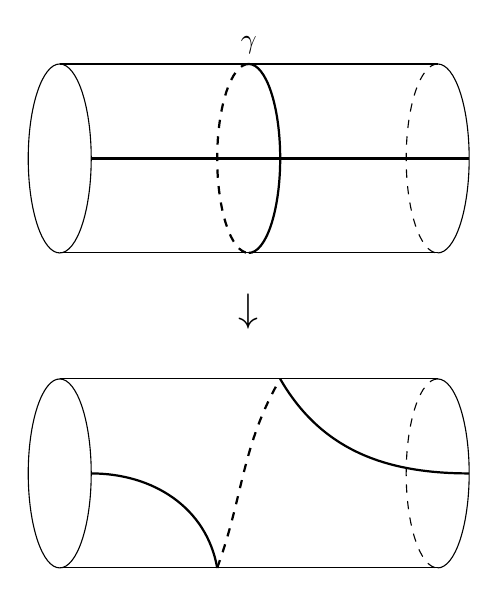
\begin{tikzpicture}[scale=0.8]
            \draw (0,0+5)--(6,0+5);
            \draw (0,3+5)--(6,3+5);

            \draw[thick] (0.5, 1.5+5)--(6.5, 1.5+5);

            \draw (0, 1.5+5) circle[x radius=0.5, y radius=1.5];

            \draw(6, 0+5)arc(-90:90:0.5 and 1.5);
            \draw[dashed](6, 3+5)arc(90:270:0.5 and 1.5);

            \draw[thick](3, 0+5)arc(-90:90:0.5 and 1.5);
            \draw[thick, dashed](3, 3+5)arc(90:270:0.5 and 1.5);


            % notation
            \draw(3, 3+5) node[above]{$\gamma$};

            \draw(3, -0.5+5) node[below]{\Large$\downarrow$};


            \draw (0,0)--(6,0);
            \draw (0,3)--(6,3);

            \draw (0, 1.5) circle[x radius=0.5, y radius=1.5];

            \draw(6, 0)arc(-90:90:0.5 and 1.5);
            \draw[dashed](6, 3)arc(90:270:0.5 and 1.5);

            \draw[thick](0.5, 1.5) to[out=0,in=100](2.5, 0);
            \draw[thick, dashed](2.5, 0) to[out=70,in=-120](3.5, 3);
            \draw[thick](3.5, 3) to[out=-60,in=180](6.5, 1.5);
        \end{tikzpicture}
    \end{displaymath}
    \caption{The Dehn twist $t_\gamma$ along a simple loop $\gamma$.}
    \label{fig:Dehn-twist}
\end{figure}


Similarly, the half twist along a simple arc is defined as follows. Given a simple arc $\gamma$ on $\Sigma$, choose an orientation-preserving embedding $i \colon D \to \Sigma$ of the unit disk $D = \{z \in \bC \mid |z| \leq 1\}$ satisfying $i(t - 1/2) = \gamma(t)$ for all $t \in [0, 1] \subset D$.
Then we define the \emph{half twist along $\gamma$} to be the homeomorphism $h_\gamma \colon \Sigma \to \Sigma$ (or its mapping class) satisfying
\begin{equation}
    h_\gamma(x) = \begin{cases}
        i(z \cdot e^{2\pi \sqrt{-1} |z|}) & (x = i(z) \in i(D)),           \\
        x                                 & (x \in \Sigma \setminus i(D)),
    \end{cases}
\end{equation}
which is illustrated in Figure \ref{fig:half-twist}.
Its mapping class is also determined by the isotopy class of $\gamma$.



\begin{figure}[h]
    \centering
    \begin{displaymath}
        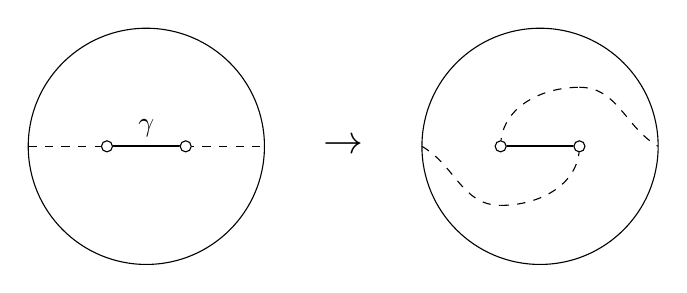
\begin{tikzpicture}
            \draw (0, 1.5) circle[radius=1.5];
            \draw[thick] (-0.5, 1.5)--(0.5, 1.5);
            \draw[dashed] (-1.5, 1.5)--(-0.5, 1.5);
            \draw[dashed] (0.5, 1.5)--(1.5, 1.5);

            \foreach \u in {-0.5, 0.5}
                {
                    \filldraw[white] (\u, 1.5) circle (2pt);
                    \draw[black] (\u, 1.5) circle (2pt);
                }
            \draw(0, 1.5) node[above]{$\gamma$};

            \draw(2.5, 1.5) node{\Large$\rightarrow$};

            \draw (0+5, 1.5) circle[radius=1.5];
            \draw[thick] (-0.5+5, 1.5)--(0.5+5, 1.5);

            \draw[dashed](-1.5+5, 1.5) to[out=-30,in=180](-0.5+5, 0.75);
            \draw[dashed](-0.5+5, 0.75) to[out=0,in=-90](0.5+5, 1.5);

            \draw[dashed](-0.5+5, 1.5) to[out=90,in=180](0.5+5, 2.25);
            \draw[dashed](0.5+5, 2.25) to[out=0,in=150](1.5+5, 1.5);


            \foreach \u in {-0.5, 0.5}
                {
                    \filldraw[white] (\u+5, 1.5) circle (2pt);
                    \draw[black] (\u+5, 1.5) circle (2pt);
                }
        \end{tikzpicture}
    \end{displaymath}
    \caption{The half twist $h_\gamma$ along a simple arc $\gamma$.}
    \label{fig:half-twist}
\end{figure}



\subsection{The actions of mapping class groups on the fundamental groups}
Let $\Sigma$, $\partial \Sigma$, and $P$ be as above.
Assume $\Sigma$ is connected, and fix a base point $x \in \Sigma \setminus (P \cup \partial \Sigma)$.
A homeomorphism $f \colon \Sigma \to \Sigma$ fixing $P$ as a set induces an isomorphism $f_* \colon \pi_1(\Sigma \setminus P, x) \to \pi_1(\Sigma \setminus P, f(x)), $ which in turn induces an automorphism $[E] \mapsto [\gamma_{-1} * f(E) * \gamma]$ of $\pi_1(\Sigma \setminus P, x) = \pi_1(\Sigma \setminus P)$ by choosing a path $\gamma$ from $x$ to $f(x)$.
The class of this automorphism in $\Out(\pi_1(\Sigma \setminus P)) \coloneqq \Aut(\pi_1(\Sigma \setminus P))/\Inn(\pi_1(\Sigma \setminus P))$, where $\Inn(\pi_1(\Sigma \setminus P))$ is the inner automorphism group of $\pi_1(\Sigma \setminus P)$, does not depends on the choice of $\gamma$, and the resulting group homomorphism will be denoted by
\begin{equation}
    \sigma \colon \MCG^{\pm}(\Sigma, P) \to \Out(\pi_1(\Sigma \setminus P)).
\end{equation}
There is the following remarkable theorem for this map.
\begin{theorem}[Dehn--Nielsen--Baer theorem, {\cite[Theorem 8.8]{MR2850125}}]\label{thm:Dehn--Nielsen--Baer}
    Let $\Out^\star(\pi_1(\Sigma \setminus P))$ be the subgroup of $\Out(\pi_1(\Sigma \setminus P))$
    consisting of the elements that preserve the set of conjugacy classes of the simple closed curves surrounding each point in $P$.
    If $\partial \Sigma = \emptyset$ and $\chi(\Sigma \setminus P)<0$, then the natural map
    \begin{equation}
        \sigma \colon \MCG^{\pm}(\Sigma, P) \to \Out^\star(\pi_1(\Sigma \setminus P))
    \end{equation}
    is an isomorphism.
\end{theorem}
We will use the injectivity of $\sigma$ to identify certain elements of mapping class groups.








\section{Fourier--Mukai transforms and twist functors}\label{section:fourier-mukai-transforms-and-twist-functors}
\subsection{Fourier--Mukai transforms}\label{subsection:fourier-mukai-transforms}
Let $T$, $X$, and $Y$ be schemes.
Let\ $p \colon X \to T$ and $q \colon Y \to T$ be flat and separated morphisms.
For an object $\cP \in D_{qc}(X \times_T Y)$, we define the \emph{(relative) integral functor $\Phi_{\cP} = \Phi^{X \to Y}_P \colon D_{qc}(X) \to D_{qc}(Y)$ with kernel $\cP$} by
\begin{equation}
    \Phi_{\cP}(-) = \pi_{Y*}(\pi_{X}^*(-) \otimes \cP),
\end{equation}
where $\pi_X \colon X \times_T Y \to X$ and $\pi_Y \colon X \times_T Y \to Y$ be the natural projections.
If an integral functor $\Phi_{\cP}$ is an equivalence, then we call $\Phi_{\cP}$ a \emph{Fourier--Mukai transform} and $\cP$ a \emph{Fourier--Mukai kernel}.

\begin{example}
    \begin{enumerate}
        \item Let $f \colon X \to Y$ be a morphism of $T$-schemes. Let $\Gamma \subset X \times_T Y$ be the graph of $f$ and $\overline{\Gamma} \subset Y \times_T X$ be its transpose. Then we have $f_* \cong \Phi_{\cO_{\Gamma}} \colon D_{qc}(X) \to D_{qc}(Y)$ and $f^* \cong \Phi_{\cO_{\overline{\Gamma}}} \colon D_{qc}(Y) \to D_{qc}(X)$.
        \item Let $L \in \Pic(X)$ be a line bundle on $X$ and $\Delta = \Delta_T \colon X \to X \times_T X$ be the diagonal morphism. Then we have $L \otimes (-) \cong \Phi_{\Delta_*L} \colon D_{qc}(X) \to D_{qc}(X)$.
    \end{enumerate}
\end{example}

The composition $\Phi_{\cQ} \circ \Phi_{\cP} \colon D_{qc}(X) \to D_{qc}(Z)$ of two integral functors $\Phi_{\cP} \colon D_{qc}(X) \to D_{qc}(Y)$ and $\Phi_{\cQ} \colon D_{qc}(Y) \to D_{qc}(Z)$  is isomorphic to an integral functor $\Phi_{\cQ * \cP}$, where the kernel $\cQ * \cP \in D_{qc}(X \times_T Z)$ is the \emph{convolution} of $P$ and $Q$ defined as follows:
\begin{equation}
    \cQ * \cP = \pi_{XZ*}(\pi_{XY}^*\cP \otimes \pi_{YZ}^*\cQ).
\end{equation}
Here $\pi_{XY}$, $\pi_{YZ}$, and $\pi_{XZ}$ are the natural projections from $X \times_T Y \times_T Z$ to $X \times_T Y$, $Y \times_T Z$, and $X \times_T Z$, respectively.

The adjoint functors to an integral functor are also given by integral functors under a mild finiteness assumption.
\begin{theorem}[{\cite{MR3720794}}]\label{thm:adjoint-to-integral-functors}
    Let $T$ be a noetherian scheme.
    Let $p \colon X \to T$ and $q \colon Y \to T$ be flat and separated morphisms of finite type, and let $\cP \in D^b(X \times_T Y)$.
    \begin{enumerate}
        \item Suppose that $Y$ is quasi-projective over $T$. If $\cP$ is $\pi_X$-perfect and has proper support over $X$, then the integral functor $\Phi_{\cP_L} \colon D_{qc}(Y) \to D_{qc}(X)$ with the kernel $\cP_L = \CHom(\cP, \pi_X^!\cO_X)$ is the left adjoint functor to $\Phi_{\cP}$.
        \item Suppose that $X$ is quasi-projective over $T$. If $\cP$ is $\pi_Y$-perfect and has proper support over $Y$, then the integral functor $\Phi_{\cP_R} \colon D_{qc}(Y) \to D_{qc}(X)$ with the kernel $\cP_R = \CHom(\cP, \pi_Y^!\cO_Y)$ is the right adjoint functor to $\Phi_{\cP}$.
    \end{enumerate}
\end{theorem}


We will mainly focus on the case where $X = Y$, $p = q$, and $\Phi_{\cP}$ an equivalence (i.e.~ a Fourier--Mukai transform).
Let us introduce the group of invertible integral kernels $\FM_T(X)$.
By projection formula we have $\cP * \cO_{\Delta} \cong \cP \cong \cO_{\Delta} * \cP$ for the structure sheaf $\cO_{\Delta} = \Delta_{T*}\cO_X$ of the diagonal $\Delta_T \colon X \hookrightarrow X \times_T X$ and any complex $\cP \in D_{qc}(X \times_T X)$.
This means that $\cO_{\Delta}$ is the unit element for the convolution.
We can also check that the convolution is associative.
Based on these observations we give the following definition.
\begin{definition}
    Let $T$ be a scheme and $X \to T$ be a flat separated morphism.
    The group of Fourier--Mukai kernels $\FM_T(X)$ is
    \begin{equation}
        \FM_T(X) \coloneqq \{\cP \in D_{qc}(X \times_T X) \mid \text{$\cP$ is invertible w.r.t.~ the convolution}\}/\cong
    \end{equation}
    with the group operation being the convolution.
\end{definition}

There is a natural homomorphism to the group of autoequivalences of $D_{qc}(X)$
\begin{equation}\label{eq:FM-to-Auteq}
    \FM_T(X) \to \Auteq(D_{qc}(X)), \quad \cP \mapsto \Phi_{\cP}
\end{equation}
by definition.
In a nice situation, the functor $\Phi_{\cP}$ restricts to an autoequivalence of the full subcategory $D^b(X) \subset D_{qc}(X)$ and the map $\cP \mapsto \Phi_{\cP}$ is injective by the following claims.
\begin{lemma}[{\cite[Proposition 7.4]{MR3861804}}]
    Let $X$ be a noetherian scheme that has enough locally free sheaves (e.g.~ quasi-projective over a field).
    Then every autoequivalence $\Phi \in \Auteq D_{qc}(X)$ preserves the full subcategory $D^b(X) \subset D_{qc}(X)$.
\end{lemma}
\begin{lemma}[{\cite[Theorem 1.5]{MR3556457}}]\label{lem:uniqueness-of-FM-kernel}
    Let $k$ be a field and $X$ be a quasi-projective scheme over $k$.
    Then for every Fourier--Mukai transform $\Phi_{\cP} \colon D^b(X) \xrightarrow{\sim} D^b(X)$ the kernel $\cP \in D_{qc}(X \times_k X)$ is unique up to isomorphism.
\end{lemma}
\begin{proposition}\label{prop:FM-to-Auteq}
    Let $k$ be a field and $X$ be a quasi-projective scheme over $k$.
    Then there is an injective group homomorphism
    \begin{equation}
        \FM_k(X) \hookrightarrow \Auteq(D^b(X)), \quad \cP \mapsto \Phi_{\cP}.
    \end{equation}
\end{proposition}
\begin{proof}
    It follows from the previous two lemmas.
\end{proof}

The next proposition describes the behavior of Fourier--Mukai transforms when we forget the base.
\begin{proposition}\label{prpo:forget-base}
    Let $T \to S$ be a flat separated morphism of schemes.
    Then there is an injective group homomorphism
    \begin{equation}
        \FM_T(X) \hookrightarrow \FM_S(X), \quad \cP \mapsto \iota_* \cP,
    \end{equation}
    where $\iota \colon X \times_T X \to X \times_S X$ is the natural morphism.
    In addition, the following diagram is commutative:
    \[
        \begin{tikzcd}
            \FM_T(X) \ar[r, "\iota_*"] \ar[rd, out=-90, in=180, "\Phi_{(-)}"'] & \FM_S(X) \ar[d, "\Phi_{(-)}"] \\
            & \Auteq(D_{qc}(X)).
        \end{tikzcd}
    \]
\end{proposition}
\begin{proof}
    First of all, we note that $\iota \colon X \times_T X \to X \times_S X$ is a closed immersion, since there is a cartesian diagram
    \[
        \begin{tikzcd}
            X \times_T X \ar[r] \ar[d, "\iota"'] & T \ar[d, "\Delta"]\\
            X \times_S X \ar[r] & T \times_S T
        \end{tikzcd}
    \]
    and $T \to S$ is separated.


    Let $\Delta_T \colon X \to X \times_T X$ and $\Delta_S \colon X \to X \times_S X$ be the diagonal morphisms.
    For every $\cP, \cQ \in D_{qc}(X \times_T X)$ we have $\iota_*(\cP * \cQ) \cong (\iota_* \cP) * (\iota_* \cQ)$ by projection formula. We also have $\iota_* \Delta_{T*}\cO_X \cong \Delta_{S*}\cO_X$.
    Thus, there is a well-defined group homomorphism  $\FM_T(X) \to \FM_S(X), \cP \mapsto \iota_* \cP$.
    To show that it is injective, let $\cP \in \FM_T(X)$ and assume $\iota_* \cP \cong \Delta_{S*}\cO_X$.
    Since $\iota$ is a closed immersion, the isomorphism $\iota_* \cP \cong \Delta_{S*}\cO_X \cong \iota_*\Delta_{T*}\cO_X$ implies that $\cP$ is a coherent sheaf and hence $\cP \cong \Delta_{T*}\cO_X$, which means that the homomorphism is injective.

    The commutativity of the last diagram follows from the projection formula.
\end{proof}

The following result says that relative Fourier--Mukai transforms are compatible with base change.
Especially, we can ``restrict'' them to (the derived category of) each fiber of $X \to T$.
This kind of construction has appeared in the literature such as \cite{MR2238172, MR2505443, MR2593258} and will play a central role in our arguments.
We give a formulation that applies to our setting.
\begin{proposition}\label{prop:restriction-to-fiber}
    Let $T' \to T$ be a morphism of schemes and $X' = X \times_T T'$ be the fiber product.
    Let $f \colon X' \to X$ and $\varphi \colon X' \times_{T'} X' \to X \times_T X$ be the natural morphisms.
    Then we have a group homomorphism
    \begin{equation}
        \FM_T(X) \to \FM_{T'}(X'), \quad \cP \mapsto \varphi^* \cP.
    \end{equation}
    Moreover, the Fourier--Mukai transforms $\Phi_{\cP}$ and $\Phi_{\varphi^* \cP}$ fit into the following commutative diagram:
    \begin{equation}\label{diagram:restriction-to-fiber}
        \begin{tikzcd}
            D_{qc}(X') \ar[r, "f_*"] \ar[d, "\Phi_{\varphi^* \cP}"'] & D_{qc}(X) \ar[r, "f^*"]\ar[d, "\Phi_{\cP}"] & D_{qc}(X') \ar[d,  "\Phi_{\varphi^* \cP}"]\\
            D_{qc}(X') \ar[r, "f_*"'] & D_{qc}(X) \ar[r, "f^*"'] & D_{qc}(X').
        \end{tikzcd}
    \end{equation}
\end{proposition}
\begin{proof}
    Let $\Delta \colon X \to X \times_T X$ and $\Delta' \colon X' \to X' \times_{T'} X'$ be the diagonal morphisms.
    We need to show that
    \begin{enumerate}
        \item $(\varphi^* \cP) * (\varphi^* \cQ) \cong \varphi^*(\cP * \cQ)$ for $\cP, \cQ \in D_{qc}(X \times_T X)$ and
        \item $\varphi^*\Delta_{T*}\cO_X \cong \Delta'_{T'*}\cO_{X'}$.
    \end{enumerate}
    Let $\psi \colon X' \times_{T'} X' \times_{T'} X' \to X \times_T X \times_T X$ be the natural morphism.
    For $i, j \in \{1, 2, 3\}$ let $\pi_{ij} \colon X \times_T X \times_T X \to X \times_T X$ and $p_{ij} \colon X' \times_{T'} X' \times_{T'} X' \to X \times_{T'} X'$ be the natural projections to the $(i, j)$ components.
    Then for $P, Q \in D_{qc}(X \times_T X)$ we have
    \begin{align}
        (\varphi^* \cP) * (\varphi^* \cQ) & =p_{13*}(p_{12}^* \varphi^* \cP \otimes p_{23}^* \varphi^* \cQ)   \\
                                          & \cong p_{13*}(\psi^*\pi_{12}^* \cP \otimes \psi^* \pi_{23}^* \cQ) \\
                                          & \cong p_{13*}\psi^*(\pi_{12}^* \cP \otimes \pi_{23}^* \cQ)        \\
                                          & \cong \varphi^*\pi_{13*}(\pi_{12}^* \cP \otimes \pi_{23}^* \cQ)   \\
                                          & = \varphi^*(\cP * \cQ),
    \end{align}
    where $p_{13*}\psi^* \cong \varphi^*p_{13*}$ holds by tor-independence of the diagram
    \[
        \begin{tikzcd}
            X' \times_{T'} X' \times_{T'} X' \ar[r, "\psi"] \ar[d, "p_{13}"] &  X \times_{T} X \times_{T} X \ar[d, "\pi_{13}"] \\
            X' \times_{T'} X' \ar[r, "\varphi"] & X \times_{T} X.
        \end{tikzcd}
    \]
    The second claim (2) follows from the tor-independent base change for the cartesian diagram (Lemma \ref{lem:tor-independent-situations}(2))
    \[
        \begin{tikzcd}
            X' \ar[r] \ar[d, "\Delta'"] &  X \ar[d, "\Delta"] \\
            X' \times_{T'} X' \ar[r] & X \times_{T} X.
        \end{tikzcd}
    \]
    Finally, the commutativity of the last diagram \eqref{diagram:restriction-to-fiber} is a consequence of a standard argument using the projection formula and flat base change.
\end{proof}

We present a criterion to determine when a kernel $\cP \in D_{qc}(X \times_T X)$ belongs to $\FM_T(X)$.
Roughly speaking, this criterion says it is enough to check that $\Phi_{\cP}$ is an equivalence and whose left (or, equivalently, right) adjoint is also an integral functor.
It will be used combined with Theorem \ref{thm:adjoint-to-integral-functors}.
\begin{lemma}\label{lem:criterion-for-invertible-kernel}
    Let $X \to T \to \Spec k$ be morphisms of schemes in which
    \begin{itemize}
        \item $k$ is a field,
        \item $T \to \Spec k$ is separated,
        \item $X \to T$ is flat, and
        \item $X \to \Spec k$ is quasi-projective.
    \end{itemize}
    Let $\cP \in D_{qc}(X \times_T X)$ and suppose that $\Phi_{\cP} \colon D_{qc}(X) \to D_{qc}(X)$ has a left (or right) adjoint that is also an integral functor $\Phi_{\cQ}$ (with kernel $\cQ \in D_{qc}(X \times_T X)$).
    Then the following are equivalent:
    \begin{enumerate}
        \item $\cP$ is an element of $\FM_T(X)$.
        \item $\Phi_{\cP} \colon D_{qc}(X) \to D_{qc}(X)$ is an equivalence.
        \item $\Phi_{\cP}$ preserves $D^b(X) \subset D_{qc}(X)$ and $\Phi_{\cP} \colon D^b(X) \to D^b(X)$ is an equivalence.
    \end{enumerate}
\end{lemma}
\begin{proof}
    (1) $\Rightarrow$ (2) is clear.
    (2) $\Rightarrow$ (3) follows from Proposition \ref{prop:FM-to-Auteq}.

    We will show (3) $\Rightarrow$ (1).
    Note that $X \to T$ and $T \to \Spec k$ are automatically flat and separated.
    We only discuss the case where $\Phi_{\cQ}$ is the left adjoint to $\Phi_{\cP}$ (the right adjoint case is similar).
    Let $\iota \colon X \times_T X \hookrightarrow X \times_k X$ be the natural inclusion.
    By the assumption and the proof of Proposition \ref{prpo:forget-base} we have
    \begin{equation}
        \Phi_{\iota_*(\cP * \cQ)} \cong \Phi_{\iota_* \cP} \circ \Phi_{\iota_* \cQ} \cong \id \cong \Phi_{\Delta_{k*}\cO_X} \cong \Phi_{\iota_*\Delta_{T*}\cO_X} \colon D^b(X) \to D^b(X).
    \end{equation}
    Then $\iota_*(\cP * \cQ) \cong \iota_*\Delta_{T*}\cO_X$ holds by Lemma \ref{lem:uniqueness-of-FM-kernel} and again by the proof of Proposition \ref{prpo:forget-base} we have $\cP * \cQ \cong \Delta_{T*}\cO_X$.
    Similarly, we have $\cQ * \cP \cong \Delta_{T*}\cO_X$, and we obtain $\cP \in \FM_T(X)$.
\end{proof}


Finally, we close this subsection by giving the following useful lemma.
It is well-known for smooth projective cases (see {\cite[3.3]{MR3713877}}, for instance).
We give a proof which applies to quasi-projective and not necessarily smooth varieties.

\begin{lemma}\label{lem:criterion-to-be-standard-functor}
    Let $k$ be an algebraically closed field of characteristic zero.
    Let $X$ and $Y$ be connected quasi-projective schemes over $k$.
    Let $\cP \in D^b(X \times Y)$ be an object whose support is proper over $X$.
    Suppose that the integral functor $\Phi = \Phi_{\cP}$ satisfies the following condition: For any closed point $x \in X$, there exists a closed point $y \in Y$ and an integer $n_x$ such that $\Phi(\cO_x) \cong \cO_y[n_x]$.
    Then there exists a morphism $\varphi \colon X \to Y$, line bundles $L_1 \in \Pic X$, $L_2 \in \Pic Y$, and an integer $n$ such that $\Phi \cong L_2 \otimes \varphi_*(L_1 \otimes -)[n]$.
\end{lemma}
\begin{proof}
    We repeat the proof of \cite[Lemma 2.14]{MR2155085}.
    Let $\pi_X \colon X \times Y \to X$ and $\pi_Y \colon X \times Y \to Y$ be the natural projections and $i_x \colon \{x\} \times Y \hookrightarrow X \times X$ be the natural inclusion for each closed point $x \in X$.
    From $i_x^*(\cP) \cong \cO_{(x, y)}[n_x]$, which follows from the assumption, we conclude that the complex $\cP$ is a shift of coherent sheaf on $X \times Y$ and flat over $X$ (\cite[Lemma 4.3]{MR1651025}).
    By Lemma \ref{lem:degree-is-locally-constant} below $x \mapsto n_x$ is a locally constant function on the set of closed points of $X$,
    and hence constant since we assumed $X$ to be connected.
    Therefore we may assume $n_x=0$ for every $x \in X$ with appropriate shift and $\cP$ is just a coherent sheaf on $X \times Y$ flat over $X$.

    From here to the end of the proof, the symbols such as $\pi_{X*}$ or $i_*$ denote \emph{non-derived functors}.
    Let $i \colon Z \hookrightarrow X \times Y$ be the schematic support of $P$ and $p_X = \pi_X \circ i$ be the projection to $X$.
    Note that $\cP \cong i^*i_* \cP = i_*(\cP\vert_Z)$ holds under our notations here.
    First, We claim that the canonical morphism
    \begin{equation}\label{eq:canonical_surjection}
        \pi_X^* \pi_{X*}(\cP \otimes \pi_Y^*\cO_X(d)) \to \cP \otimes \pi_Y^*(\cO_X(d))
    \end{equation}
    is surjective for sufficiently large $d$, where $\cO_X(d) = \cO_X(1)^{\otimes d}$ is the multiple of a fixed very ample line bundle on $X$.
    Since the support $Z$ is proper over $X$ and both of them are quasi-projective, the morphism $p_X \colon Z \to X$ is projective. The sheaf $\pi_Y^*\cO_X(1)\vert_Z \eqqcolon \cO_{Z/X}(1)$ gives a very ample line bundle on $Z$ relative to $X$. Therefore we have a surjection
    \begin{equation}
        p_X^* p_{X*}(\cP\vert_Z \otimes \cO_{Z/X}(d)) \to \cP\vert_Z \otimes \cO_{Z/X}(d)
    \end{equation}
    for large $d$ by \cite[Theorem III 8.8]{MR0463157}.
    By taking its push-forward $i_*$ and using the projection formula, there is a surjective morphism
    \begin{equation}\label{eq:canonical_surjection_2}
        i_*i^*\pi_X^* \pi_{X*}(\cP \otimes \pi_Y^*\cO_X(d)) \to \cP \otimes \pi_Y^*(\cO_X(d)).
    \end{equation}
    Our claim follows from \eqref{eq:canonical_surjection_2} and the surjection $\id \to i_*i^*$.


    By the projection formula we have $\pi_{X*}(\cP \otimes \pi_Y^* \cO_X(d)) \cong p_{X*}(P\vert_Z \otimes \cO_{Z/X}(d))$ and the latter is a locally free sheaf for large $d$
    because $p_X \colon Z \to X$ is projective and $\cP\vert_Z$ is flat over $X$.
    It has rank one by
    \begin{equation}
        \pi_{X}(\cP \otimes \pi_Y^* \cO_X(d))\vert_{\{x\}} \cong H^0((\cP \otimes \pi_Y^* \cO_X(d))\vert_{\{x\} \times Y}) \cong H^0(\cO_{(x, y)}) \cong k,
    \end{equation}
    where the first isomorphism is flat base change and the second follows from $i_x^*(\cP) \cong \cO_{(x, y)}$.
    Therefore the surjection \eqref{eq:canonical_surjection} gives rise to the surjection
    \begin{equation}\label{eq:surjection}
        \cO_{X \times Y} \to \cP \otimes \pi_X^*L^\vee \otimes \pi_Y^*(\cO_X(d)),
    \end{equation}
    in which $L$ denotes the line bundle $\pi_{X*}(\cP \otimes \pi_Y^* \cO_X(d))$.
    The sheaf $\cP \otimes \pi_X^*L^\vee \otimes \pi_Y^*(\cO_X(d))$ is flat over $X$ and there is an isomorphism
    \begin{equation}
        (P \otimes \pi_X^*L^\vee \otimes \pi_Y^*(\cO_X(d)))\vert_{x \times Y} \cong \cO_{(x, y)}.
    \end{equation}
    It means that the surjection \eqref{eq:surjection} gives rise to a morphism $\varphi \colon X \to \Hilb_{Y}^1$ and \eqref{eq:surjection} is identified with the pullback of the universal quotient
    \begin{equation}
        (\varphi \times \id)^*(\cO_{\Hilb_{Y}^1 \times Y} \to \cU).
    \end{equation}
    Under the identification $Y \cong \Hilb_{Y}^1$ and $\cU \cong \cO_{\Delta_{Y}}$ we have
    \begin{align}
        \cP & \cong (\varphi \times \id)^*\cO_{\Delta_{Y}} \otimes \pi_X^*L \otimes \pi_Y^*(\cO_X(d))^\vee \\
            & \cong \cO_{\Gamma_\varphi} \otimes \pi_X^*L \otimes \pi_Y^*(\cO_X(d))^\vee,
    \end{align}
    where $\Gamma_\varphi$ is the graph of $\varphi$.
    This concludes the proof.
\end{proof}

\begin{lemma}\label{lem:degree-is-locally-constant}
    Let $k$ be an algebraically closed field of characteristic zero.
    Let $X$ and $Y$ be schemes of finite type over $k$ and $\cP \in D^b(X \times Y)$ be an object whose support is proper over $X$.
    Let $i_x \colon \{x\} \times Y \hookrightarrow X \times Y$ be the natural inclusion for a closed point $x \in X$.
    Then the set
    \begin{equation}
        \left\{x \in X \mid x\text{ is a closed point, }\cH^m(i_x^*\cP) = 0 \text{ unless } m \neq 0\right\}
    \end{equation}
    is the set of closed points of an open subset of $X$.
\end{lemma}
\begin{proof}
    If $Y$ is proper over $k$, then the claim is a special case of \cite[Lemma 3.1.6]{Bridgeland2002FourierMukaiTF}.
    For general $Y$, we take a compactification of $Y$, i.e.~ a proper scheme $\overline{Y}$ over $k$ with an open immersion $\iota \colon Y \hookrightarrow \overline{Y}$.
    We can always find such $\overline{Y}$ by Nagata's compactification theorem.
    Then we have cartesian squares
    \[
        \begin{tikzcd}
            \{x\} \times Y \ar[r, hookrightarrow, "\iota"] \ar[d, hookrightarrow, "i_x"] & \{x\} \times \overline{Y} \ar[r] \ar[d, hookrightarrow, "\overline{i_x}"]& \{x\} \ar[d, hookrightarrow]\\
            X \times Y \ar[r, "\id \times \iota"] & X \times \overline{Y} \ar[r] & X,
        \end{tikzcd}
    \]
    where $\overline{i_x}$ is the natural inclusion.
    The push-forward $\overline{\cP} = (\id \times \iota)_* \cP$ is an object of $D^b(X \times \overline{Y})$ by the assumption of proper support and hence the statement holds for $X$, $\overline{Y}$, and $\overline{\cP}$.
    Therefore it is enough to show the equivalence
    \begin{equation}
        \cH^m(i_x^* \cP) = 0 \Leftrightarrow \cH^m(\overline{i_x}^*(\overline{\cP})) = 0
    \end{equation}
    for every $m \in \bZ$.



    Since $\iota$ is an open immersion (and hence flat), there is the base change isomorphism $\overline{i_x}^*(\overline{\cP}) \cong \iota_*i_x^* \cP$.
    Let $j \colon Z \hookrightarrow Y \cong \{x\} \times Y$ be the schematic support of $i_x^* \cP$.
    It is proper over $k$ and $i_x^* \cP \cong j_* \cQ$ for some $\cQ \in D^b(Z)$ (\cite[\href{https://stacks.math.columbia.edu/tag/0CYK}{Tag 0CYK}]{stacks-project}).
    The inclusions $j$ and $\iota \circ j$ are closed immersions because of the properness of $Z$.
    There are isomorphisms
    \begin{equation}
        \cH^m(i_x^* \cP) \cong \cH^m(j_* \cQ) \cong j_*\cH^m(\cQ),
    \end{equation}
    \begin{equation}
        \cH^m(\overline{i_x}^*(\overline{\cP})) \cong \cH^m(\iota_*i_x^* \cP) \cong \cH^m(\iota_*j_* \cQ) \cong \iota_*j_*\cH^m(\cQ),
    \end{equation}
    and the vanishing of $j_*\cH^m(\cQ)$ and $\iota_*j_*\cH^m(\cQ)$ are both equivalent to the vanishing of $\cH^m(\cQ)$.
    It finishes the proof.
\end{proof}


\subsection{Spherical objects and twist functors}
In \cite{MR1831820}, Seidel and Thomas introduced the notion of spherical objects of derived categories and associated autoequivalences called twist functors.
This construction is an analog or a counterpart of Dehn twists along Lagrangian spheres in symplectic geometry, through homological mirror symmetry.

Let $X$ be a quasi-projective Gorenstein scheme over a field $k$ and $f \colon X \to \Spec k$ be the structure morphism.
We assume $X$ to be connected (or more generally equidimensional) with $\dim X = d$.
The dualizing complex $f^!\cO_{\Spec k}$ is of the form $\omega_X[-d]$ for some line bundle $\omega_X$ on $X$, which is called the \emph{canonical bundle} of $X$.
\begin{definition}[{\cite{MR1831820}}]
    We say $\cE \in D^b(X)$ is a \emph{($d$-)spherical object} if
    \begin{enumerate}
        \item $\cE$ is perfect and has proper support,
        \item $\cE \otimes \omega_X \cong \cE$, and
        \item $\Ext^*_X(\cE, \cE) \cong k \oplus k[-d]$.
    \end{enumerate}
\end{definition}

\begin{theorem}[{\cite{MR1831820}}]
    Let $\cE \in D^b(X)$ be a spherical object.
    Let $T_{\cE} = \Phi_{P_{\cE}}$ be the integral functor with the kernel
    \begin{equation}
        P_{\cE} = \Cone(\cE^\vee \boxtimes \cE \xrightarrow{\ev} \Delta_{k*}\cO_X),
    \end{equation}
    where the natural ``evaluation'' morphism $\ev$ is the composition of
    \begin{enumerate}
        \item the restriction $\cE^\vee \boxtimes \cE \to \Delta_{k*}(\cE^\vee \otimes \cE)$ and
        \item $\Delta_{k*}(\cE^\vee \otimes \cE) \to \Delta_{k*}\cO_X$ induced by the natural pairing $\cE^\vee \otimes \cE \to \cO_X$.
    \end{enumerate}
    Then $T_{\cE}$ is an autoequivalence of $D^b(X)$.
\end{theorem}
The autoequivalence $T_{\cE}$ is called the \emph{twist functor (or spherical twist) along $\cE$}.
We remark that there is an exact triangle
\begin{equation}
    \Ext^*_X(\cE, \cF)\otimes_k \cE \to \cF \to T_{\cE}(\cF) \xrightarrow{+1}
\end{equation}
for every $\cF \in D^b(X)$.
As an immediate consequence of this triangle, we have the following.
\begin{corollary}\label{cor:orthogonal-to-spherical}
    Let $\cF \in \langle \cE \rangle^\perp = \{\cF \mid \Ext^*_X(\cE, \cF) = 0\} \subset D^b(X)$ be an object that is right orthogonal to $\cE$ (e.g. $\Supp \cF \cap \Supp \cE = \emptyset$).
    Then $T_{\cE}(\cF) \cong \cF$.
\end{corollary}
\begin{example}[{\cite{MR1831820}}]\label{ex:spherical-objects}
    \begin{enumerate}
        \item Let $C$ be a (Gorenstein) curve. Then for any smooth point $x \in C$, its structure sheaf $\cO_x$ is spherical. There is an isomorphism $T_{\cO_x} \cong (-) \otimes \cO(x)$.
        \item Let $X$ be a strict Calabi-Yau variety, i.e.~ a smooth projective variety whose canonical bundle is trivial and satisfying $H^i(X, \cO)=0$ for $0 < i < \dim X$. Then any line bundle on $X$ is spherical.
        \item Let $S$ be a smooth surface and $G \subset S$ be a $(-2)$-curve. Then the sheaf $\cO_G(a)$, the push-forward of the line bundle of on $G \cong \bP^1$ with degree $a \in \bZ$, is spherical. This is a consequence of Hirzebruch--Riemann--Roch theorem or Proposition \ref{prop:exceptional-to-spherical}.
        \item Let $X$ be a smooth $3$-fold and $C \subset X$ be a $(-1, -1)$-curve, i.e.~ a smooth rational curve with normal bundle $N_{C/X} \cong \cO_{\bP^1}(-1)\oplus\cO_{\bP^1}(-1)$. Then the structure sheaf $\cO_C$ is spherical in $D^b(X)$.
    \end{enumerate}
\end{example}
\begin{proposition}[{\cite[Proposition 3.15]{MR1831820}}]\label{prop:exceptional-to-spherical}
    Let $X$ be a smooth quasi-projective variety and $\iota \colon Y \hookrightarrow X$ be a projective hypersurface.
    Assume $\iota^*\omega_X$ is trivial.
    If $\cE \in \Perf(Y)$ is an \emph{exceptional object} (i.e.~ $\Ext^*_X(\cE, \cE) \cong k$), then $\iota_* \cE \in D^b(X)$ is a spherical object.
\end{proposition}
\begin{example}\label{ex:spherical-object-from-K3-degeneration}
    Let $\pi \colon X \to C$ be a type \rom{3} degeneration of K3 surfaces \cite{Kulikov1977,Persson--Pinkham1981} (over $\bC$).
    It has the following properties by definition.
    \begin{enumerate}
        \item The canonical bundle $\omega_X$ of the total space $X$ is trivial.
        \item The central fiber $\iota \colon X_0 = \pi^{-1}(0) \hookrightarrow X$ is a reducible surface $X_0 = \bigcup_i V_i$, and each component $V_i$ is a complete rational surface.
    \end{enumerate}
    Additionally, we assume that $X$ and $C$ are quasi-projective and each $V_i$ is smooth.
    Then the structure sheaf $\cO_{V_i}$ of $V_i$ is an exceptional object in $\Perf(V_i)$, since the hodge numbers $h^{0,1}$ and $h^{0,2}$ of a smooth rational surface are zero.
    By the property (1) and Proposition \ref{prop:exceptional-to-spherical}, the structure sheaf $\cO_{V_i}$ is a spherical object in $D^b(X)$.
    The same argument applies to arbitrary line bundles (or exceptional objects) on $V_i$.


    % A concrete example of such situations is constructed as follows.
    % Let $S = \{F(x, y, z, w) = 0\} \subset \bP^3$ be a K3 surface defined by a homogeneous quartic polynomial $F$, and $T = \{xyzw = 0\} \subset \bP^3$ be a union of four planes.
    % For a generic choice of $F$, the pencil $\overline{X} = \{xyzw + t F(x, y, z, w) = 0\} \subset \bP^3 \times \bC$ spanned by $S$ and $T$
    % has exactly $24$ singular points on the central fiber $\overline{X_0} = T$.
    % They are the intersections of $\{F = 0\}$ and the edges of the tetrahedron $T$, and all of them are ordinary double points.
    % We can take a suitable small resolution $X \to \overline{X}$ of these singularities to obtain a type \rom{3} degeneration of K3 surfaces $\pi \colon X \to \overline{X} \to \bC$.
    % In this case the central fiber $X_0$ has four components, each of which is a blow-up of $\bP^2$ at six points.
\end{example}
The following basic properties of twist functors will be useful for us.
\begin{lemma}
    Let $\cE, \cE'$ be spherical objects in $D^b(X)$.
    \begin{enumerate}
        \item For any equivalence $\Phi \in \Auteq{D^b(X)}$, we have \begin{equation}
                  \Phi \circ T_{\cE} \circ \Phi^{-1} \cong T_{\Phi(\cE)}.
              \end{equation}
        \item If $\Ext^*_X(\cE, \cE') = 0$, then $T_{\cE}T_{\cE'} \cong T_{\cE'}T_{\cE}$.
        \item If $\dim \sum_i \Ext_X^i(\cE, \cE') = 1$, then $T_{\cE}T_{\cE'} T_{\cE} \cong T_{\cE'}T_{\cE}T_{\cE'}$.
    \end{enumerate}
\end{lemma}
\begin{proof}
    The first statement follows by definition.
    The others are part of \cite[Theorem 1.2]{MR1831820}.
\end{proof}





\section{Construction of half-spherical twists}\label{section:construction-of-half-spherical-twists}
In this section, we prove Theorem \ref{thm:main-theorem-1-half-spherical-twist} and give some examples.
\subsection{Compatibilities}
We introduce some natural morphisms and commutative diagrams of schemes that will be used in the next subsection.

\begin{definition}[relative cup product]\label{def:relative-cup-product}
    Let $f \colon X \to Y$ be a morphism of schemes. The \emph{relative cup product morphism} $$p = p_{\cF, \cG} \colon f_*\cF \otimes f_*\cG \to f_*(\cF \otimes \cG)$$ for $\cF, \cG \in D_{qc}(X)$ is the adjoint to the canonical morphism $$f^*(f_*\cF \otimes f_*\cG) \cong f^*f_*\cF \otimes f^*f_*\cG \to \cF \otimes \cG$$ which is induced from the counit morphism $f^*f_* \to \id$.
\end{definition}
\begin{proposition}\label{prop:Kunneth-and-cup-product}
    Let $k$ be a field.
    Let $f \colon X' \to X$ be a morphism of $k$-schemes and let $g = f\times f \colon X' \times_k X' \to X \times_k X$.
    Consider the commutative diagram
    \[
        \begin{tikzcd}
            X' \arrow[r,"f"]\arrow[d, "\delta"'] & X \arrow[d,"\Delta"]&\\
            X' \times_k X' \arrow[r, "g"]& X \times_k X,
        \end{tikzcd}
    \]
    where $\Delta$ and $\delta$ are the diagonal morphisms.
    Then for any $\cF, \cG \in D_{qc}(X')$, we have a commutative diagram
    \[
        \begin{tikzcd}
            f_*\cF \boxtimes f_*\cG \arrow[rr, "\text{restriction}"]\arrow[d, "\text{Kunneth formula}"', "\sim"]&&\Delta_*(f_*\cF \otimes f_*\cG)\arrow[d, "\Delta_*(\text{relaive cup product})"]\\
            g_*(\cF \boxtimes \cG) \arrow[r, "\text{restriction}"']&g_*\delta_*(\cF \otimes \cG) \arrow[r, "\sim", sloped]&\Delta_*(f_*(\cF \otimes \cG)).
        \end{tikzcd}
    \]
\end{proposition}
\begin{proof}
    By the adjunction $\Delta_X^* \dashv \Delta_{X*}$,
    the statement is equivalent to the commutativity of the upper square of the diagram
    \[
        \begin{tikzcd}
            f_*\cF \otimes f_*\cG \arrow[rr, equal]\arrow[d, "\varphi"]&&f_*\cF \otimes f_*\cG\arrow[d, "p_{\cF, \cG}"]\\
            \Delta^*g_*(\cF \boxtimes \cG) \arrow[r]\dar&\Delta^*g_*\delta_*\delta^*(\cF \boxtimes \cG) \arrow[r]\dar&f_*(\cF \otimes \cG)\dar["\sim", sloped]\\
            f_*\delta^*(\cF \boxtimes \cG) \rar & f_*\delta^*\delta_*\delta^*(\cF\boxtimes \cG) \rar & f_*\delta^*(\cF \boxtimes \cG),
        \end{tikzcd}
    \]
    where $\varphi$ is the adjoint to the Kunneth formula isomorphism and $p_{\cF, \cG}$ is the relative cup product morphism.
    The lower squares, given by the natural morphisms $\Delta^*g_* \to f_*\delta^*$,
    $\id \to \delta_*\delta^*$,
    and $\delta^*\delta_* \to \id$, are commutative for the obvious reasons.
    Then it suffices to show that the outer square of the diagram is commutative.
    We can check that
    \begin{enumerate}
        \item the bottom edge of the outer square is the identity morphism by standard arguments of adjunctions, and
        \item the left vertical morphism is identified with $p_{\cF, \cG}$ via $f_*(\cF \otimes \cG) \cong f_*\delta^*(\cF \boxtimes \cG)$, by definition of $\varphi$ and $p_{\cF, \cG}$.
    \end{enumerate}
    This finishes the proof.
\end{proof}


\begin{proposition}\label{prop:relative-cup-product-and-Grothendieck-duality}
    Let $f \colon X' \to X$ be a proper morphism between noetherian schemes.
    Then for any $\cF \in D^b(X')$ and $\cG \in D^b(X)$, we have a commutative diagram
    \[
        \begin{tikzcd}
            \CHom(f_*\cF, \cG)\otimes f_*\cF \ar[r, "\text{pairng}"] & \cG \\
            f_*\CHom(\cF, f^!\cG)\otimes f_*\cF \ar[d, "\text{relative cup product}"']\ar[u, "\text{Grothendieck duality}"]& f_*f^!\cG \ar[u, "\text{counit}"'] \\
            f_*(\CHom(\cF, f^!\cG)\otimes \cF) \ar[ru, out=0, in=-90, "\text{pairing}"'] & \quad .
        \end{tikzcd}
    \]
\end{proposition}
\begin{proof}
    By the adjunction $(-\otimes f_*\cF) \dashv \CHom(f_*\cF, -)$, the statement is equivalent to the commutativity of the diagram
    \[
        \begin{tikzcd}
            \CHom(f_*\cF, \cG) \ar[r, equal] & \CHom(f_*\cF, \cG)\\
            f_*\CHom(\cF, f^!\cG) \ar[u, "\text{Grothendieck duality}"]\ar[d]& \CHom(f_*\cF, f_*f^!\cG)\ar[u, "(\text{counit}) \circ -"']\\
            \CHom(f_*\cF, f_*(\CHom(\cF, f^!\cG)\otimes \cF)) \ar[ru, out=0, in=-90]& \quad,
        \end{tikzcd}
    \]
    and it commutes by the very definition of the isomorphism of Grothendieck duality (see Remark \ref{remark:grothendieck-duality-isomorphism}).
\end{proof}



\subsection{Construction of half-spherical twists}
Throughout this subsection, we work over an algebraically closed field $k$.
We denote the product over $k$ by $\times$ for simplicity.

Let $X$ and $T$ be smooth quasi-projective varieties and $\pi \colon X \to T$ be a flat morphism.
Let $0 \in T$ be a closed point and $i \colon X_0 = \pi^{-1}(0) \hookrightarrow X$ be the fiber over $0$.
We have a diagram
\[
    \begin{tikzcd}
        X_0 \arrow[r,"i"]\arrow[d, "\delta"'] & X \arrow[d,"\Delta_T"]\arrow[rd, bend left, "\Delta_k"]&\\
        X_0 \times X_0 \arrow[r, "j"] \ar[d]& X \times_T X\arrow[r, "\iota"] \ar[d]&X \times X \\
        \{0\} \ar[r] & T &
    \end{tikzcd}
\]
in which $j$ and $\iota$ are the natural inclusions and $\delta$, $\Delta_T$, and $\Delta_k$ are the diagonal morphisms.
We note that the two squares are cartesian.



Now we apply the results of the subsection \ref{subsection:fourier-mukai-transforms} to this situation.
We have an injective group homomorphism $\FM_k(X_0) \hookrightarrow \Auteq D^b(X_0)$ and $\FM_k(X) \hookrightarrow \Auteq D^b(X)$ by Proposition \ref{prop:FM-to-Auteq}.
The latter morphism is completed into a commutative diagram
\[
    \begin{tikzcd}
        \FM_T(X) \ar[r, "\iota_*"] \ar[rd, out=-90, in=180, "\Phi_{(-)}"'] & \FM_k(X) \ar[d, "\Phi_{(-)}"] \\
        & \Auteq(D^b(X))
    \end{tikzcd}
\]
of injective morphisms by Proposition \ref{prpo:forget-base}.
We also have a ``restriction'' morphism $\FM_T(X) \to \FM_k(X_0), \cP \mapsto j^* \cP$ by Proposition \ref{prop:restriction-to-fiber}.
Summarizing the discussion, we have the following diagram of groups:
\[
    \begin{tikzcd}
        \FM_k(X_0) \ar[d, hookrightarrow, "\Phi_{(-)}"] & \FM_T(X)\ar[l, "j^*"']\ar[r, hookrightarrow, "\iota_*"]\ar[d, hookrightarrow, "\Phi_{(-)}"] & \FM_{k}(X) \ar[ld, hookrightarrow, out=-90, in=0, "\Phi_{(-)}"]\\
        \Auteq D^b(X_0) & \Auteq D^b(X)& \quad .
    \end{tikzcd}
\]
We regard $\FM_k(X_0) \subset \Auteq D^b(X_0)$ and $\FM_T(X) \subset \FM_k(X) \subset \Auteq D^b(X)$ by the above injective morphisms.
\begin{example}
    \begin{enumerate}
        \item Let $f \colon X \to X$ be an automorphism of $X$ over $T$.
              It induces an automorphism $f_0 \colon X_0 \to X_0$ of $X_0$.
              The functors $f_*$ and $f^*$ are autoequivalences of $D^b(X)$ and in the subgroup $\FM_T(X)$. Their restrictions to $D^b(X_0)$ are $f_{0*}$ and $f_0^*$, respectively.
        \item Let $L$ be a line bundle on $X$.
              The autoequivalence $L \otimes (-)$ of $D^b(X)$ is an element of $\FM_T(X)$ and its restriction to $D^b(X_0)$ is $L\vert_{X_0} \otimes (-)$.
    \end{enumerate}
\end{example}
Next, we pick an object $\cE \in D^b(X_0)$ such that $i_*{\cE} \in D^b(X)$ becomes a spherical object.
The twist functor $T_{i_*{\cE}}$ is a Fourier--Mukai transform (i.e.~ belongs to $\FM_k(X)$) with kernel
\begin{equation}
    \cP_{\cE} = \Cone((i_*{\cE})^\vee \boxtimes (i_*{\cE}) \xrightarrow{\ev} \Delta_{k*}\cO_X).
\end{equation}
We claim that $T_{i_*{\cE}}$ is included in a smaller group $\FM_T(X) \subset \FM_k(X)$ by constructing a relative integral kernel for $T_{i_*{\cE}}$.
\begin{lemma}
    Let $\cE \in D^b(X_0)$ and $\cE' = \CHom_{X_0}(\cE, i^!\cO_X)$.
    Then we have an isomorphism
    \begin{equation}
        (i_*{\cE})^\vee \boxtimes (i_*{\cE}) \xrightarrow{\sim} \iota_*j_*(\cE' \boxtimes \cE).
    \end{equation}
\end{lemma}
\begin{proof}
    It follows from the Kunneth formula and Grothendieck duality.
\end{proof}
\begin{proposition}
    Let $\cE \in D^b(X_0)$ and $\cE' = \CHom_{X_0}(\cE, i^!\cO_X)$.
    Let $\widetilde{\ev} \in \Hom(j_*(\cE' \boxtimes \cE), \Delta_{T*}\cO_X)$ be the composition morphism
    \begin{equation}
        \widetilde{\ev} \colon j_*(\cE' \boxtimes \cE) \to j_*\delta_*(\cE' \otimes \cE)\cong \Delta_{T*}i_*(\cE' \otimes \cE) \to \Delta_{T*}\cO_X,
    \end{equation}
    where
    \begin{enumerate}
        \item $\cE' \boxtimes \cE \to \delta_*(\cE' \otimes \cE)$ is the adjoint to the natural isomorphism $\delta^*(\cE' \boxtimes \cE) \cong \cE' \otimes \cE$,
        \item $j_*\delta_* \cong \Delta_{T*}i_*$ is the natural isomorphism, and
        \item $i_*(\cE' \otimes \cE) \to \cO_X$ is the adjoint to the natural pairing $\cE' \otimes \cE \to i^!\cO_X$.
    \end{enumerate}
    Then we have a commutative diagram
    \begin{equation}
        \begin{tikzcd}\label{eq:commutative-diagram-for-evaluation-map}
            (i_*{\cE})^\vee \boxtimes (i_*{\cE})\ar[r, "\ev"] \ar[d, "\sim", sloped] & \Delta_{k*}\cO_X \ar[d, "\sim", sloped]\\
            \iota_*k_*(\cE' \boxtimes \cE) \ar[r, "\iota_*(\widetilde{\ev})"]& \iota_*\Delta_{T*}\cO_X
        \end{tikzcd}
    \end{equation}
    in $D_{qc}(X \times X)$.
\end{proposition}
\begin{proof}
    The diagram in the statement can be decomposed into the following squares:
    \[
        \begin{tikzcd}
            (i_*{\cE})^\vee \boxtimes i_*{\cE} \ar[rr]\ar[d, "\sim", sloped] &  & \Delta_{k*}((i_*{\cE})^\vee \otimes i_*{\cE}) \ar[rr]\ar[d, "\sim", sloped] &  & \Delta_{k*}(\cO_X) \ar[ddd, equal]\\
            i_*(\cE')\boxtimes i_*{\cE} \ar[rr]\ar[dd]&  & \Delta_{k*}(i_*(\cE')\otimes i_*{\cE}) \ar[dd] &  & \\
            & (A) &  & (B) & \\
            \iota_*k_*(\cE' \boxtimes \cE) \ar[r] & \iota_*k_*\Delta_{Y*}(\cE' \otimes \cE) \ar[r, "\sim"]\ar[rd, out=-90, in=180, "\sim"] & \Delta_{k*}(i_*(\cE' \otimes \cE)) \ar[rr]\ar[d, "\sim", sloped] &  & \Delta_{k*}(\cO_X) \ar[d, "\sim", sloped] \\
            &  & \iota_*\Delta_{T*}i_*(\cE' \otimes \cE) \ar[rr] &  & \iota_*\Delta_{T*}\cO_X
        \end{tikzcd}
    \]
    The square (A) is commutative by Proposition \ref{prop:Kunneth-and-cup-product} for $f = i$, $\cF = \cE'$, and $\cG = \cE$.
    The commutativity of the square (B) follows from Proposition \ref{prop:relative-cup-product-and-Grothendieck-duality} for $f = i$, $\cF = \cE$, and $\cG = \cO_X$.
    The other parts of the diagram are commutative by the functoriality.
\end{proof}

The commutative diagram \eqref{eq:commutative-diagram-for-evaluation-map} provides a candidate for the relative integral kernel of the twist functor $T_{i_*{\cE}}$.
Namely, the complex $\cP'_{\cE} \in D_{qc}(X \times_T X)$ defined by
\begin{equation}\label{eq:candidate-for-relative-integral-kernel}
    \cP'_{\cE} = \Cone(k_*(\cE' \boxtimes \cE) \xrightarrow{\widetilde{\ev}} \Delta_{T*}\cO_X)
\end{equation}
satisfies $\iota_* \cP'_{\cE} \cong \cP_{\cE}$ for the (absolute) integral kernel $\cP_{\cE}$ of the twist functor
\begin{equation}
    \cP_{\cE} = \Cone((i_*{\cE})^\vee \boxtimes (i_*{\cE}) \to \Delta_{k*}\cO_X).
\end{equation}
Therefore our remaining task is to check $\cP'_{\cE} \in \FM_T(X)$.
\begin{proposition}\label{prop:twist-functor-is-in-FM}
    The complex $\cP'_{\cE}$ of \eqref{eq:candidate-for-relative-integral-kernel} is an element of $\FM_T(X)$.
    The twist functor $T_{i_*{\cE}} \in \Auteq D^b(X)$ is an element of the subgroup $\FM_T(X)$ via identification
    \begin{equation}
        \FM_T(X) \hookrightarrow \Auteq D^b(X), \quad \cP'_{\cE} \mapsto \Phi_{\cP'_{\cE}} = T_{i_*{\cE}}.
    \end{equation}
\end{proposition}
\begin{proof}
    By Theorem \ref{thm:adjoint-to-integral-functors} and Lemma \ref{lem:criterion-for-invertible-kernel}, it suffices to show that $\cP'_{\cE}$ is in $D^b(X \times_T X)$, $\pi_1$-perfect, and has proper support with respect to $\pi_1 \colon X \times_T X \to X$.
    As these conditions have the two-out-of-three property it is enough to examine $k_*(\cE' \boxtimes \cE)$ and $\Delta_{T*}\cO_X$.

    The coherent sheaf $\Delta_{T*}\cO_X$ is clearly in $D^b(X \times_T X)$ and has proper support over $X$.
    It is also $\pi_1$-perfect, since $\cO_X$ is perfect and $\Delta_{T}$ is proper (Proposition \ref{prop:proper-push-forward-of-f-perfect}).

    The isomorphism $\iota_*(k_*(\cE' \boxtimes \cE)) \cong (i_*{\cE})^\vee\boxtimes (i_*{\cE})$ tells us that $k_*(\cE' \boxtimes \cE)$ is in $D^b(X \times_T X)$ and has proper support over $X$, since a closed immersion preserves cohomologies.
    To show that $k_*(\cE' \boxtimes \cE)$ is $\pi_1$-perfect, we use Proposition \ref{prop:crirtion_for_relative_perfection}.
    Let $\cF \in D^b(X)$.
    We have
    \begin{align}
        \iota_*(k_*(\cE' \boxtimes \cE) \otimes \pi_1^*\cF) & \cong \iota_*k_*((\cE' \otimes i^*\cF) \boxtimes \cE)  \\
                                                            & \cong i_*(\cE' \otimes i^*\cF) \boxtimes i_*{\cE}      \\
                                                            & \cong (i_*(\cE') \otimes \cF) \boxtimes i_*{\cE}       \\
                                                            & \cong ((i_*{\cE})^\vee \otimes \cF) \boxtimes i_*{\cE}
    \end{align}
    in $D_{qc}(X \times_k X)$.
    The last term is a bounded complex with coherent cohomologies and thus $k_*(\cE' \boxtimes \cE) \otimes \pi_1^*\cF \in D^b(X \times_T X)$.
    By Proposition \ref{prop:crirtion_for_relative_perfection} we conclude that $k_*(\cE' \boxtimes \cE)$ is $\pi_1$-perfect.
\end{proof}
Finally, we define the half-spherical twist $H_{\cE} \in \Auteq D^b(X_0)$ along $E$ to be the ``restriction to fiber'' of the twist $T_{i_*{\cE}}$.
\begin{definition}[half-spherical twist]\label{def:half-spherical-twist}
    Let $\cE \in D^b(X_0)$ be an object such that $i_*{\cE} \in D^b(X)$ is a spherical object.
    The \emph{half-spherical twist $H_{\cE}$} along $\cE$ is the autoequivalence of $D^b(X_0)$ defined by
    \[
        \begin{tikzcd}
            \FM_k(X_0) \ar[d, phantom, sloped, "\subset"] & \FM_T(X)\ar[l, "j^*"']\ar[d, phantom, sloped, "\subset"] & j^*\cP'_{\cE} \ar[d, mapsto]& \cP'_{\cE} \ar[l, mapsto] \ar[d, mapsto]\\
            \Auteq D^b(X_0) & \Auteq D^b(X) & H_{\cE} & T_{i_*{\cE}},
        \end{tikzcd}
    \]
    where the morphism $j^*$ is the one in Proposition \ref{prop:restriction-to-fiber}.
\end{definition}
\begin{corollary}\label{cor:compatibility-of-half-spherical-twists-and-spherical-twists}
    The half-spherical twist $H_{\cE}$ and the spherical twist $T_{i_*{\cE}}$ fit into the commutative diagram
    \begin{equation}
        \begin{tikzcd}
            D^b(X_0) \ar[r, "i_*"] \ar[d, "H_{\cE}"'] & D^b(X) \ar[r, "i^*"]\ar[d, "T_{i_*{\cE}}"] & D^b(X_0) \ar[d,  "H_{\cE}"]\\
            D^b(X_0) \ar[r, "i_*"'] & D^b(X) \ar[r, "i^*"'] & D^b(X_0).
        \end{tikzcd}
    \end{equation}
\end{corollary}
\begin{proof}
    This is a direct consequence of the diagram \eqref{diagram:restriction-to-fiber} in Proposition \ref{prop:restriction-to-fiber}.
    Note that we can replace $D_{qc}$ by $D^b$, since $i_*$ is exact and $X$ is smooth.
\end{proof}

\begin{remark}
    Since the autoequivalence $H_{\cE}$ depends not only on (the isomorphism class of) $\cE$ but also on the data $(X, T, \pi, i \colon X_0 \hookrightarrow X)$, the notation $H_{\cE}$ is not precise.
    % We will later provide an example where the same $\cE$ results in different half-spherical twists, depending on the embedding $i$.
    However, we will use it for simplicity when there is no risk of confusion.
\end{remark}


\begin{example}\label{ex:half-spherical-twist-from-kodaira-fiber}
    Let $\pi \colon S \to C$ be a relatively minimal elliptic surface and $i_* \colon X_0 \hookrightarrow S$ be a reducible fiber.
    For any irreducible component $G \subset X_0$ and an integer $a \in \bZ$, the sheaf $\cO_G(a) \in D^b(X_0)$ induces a spherical object $i_*\cO_G(a)=\cO_G(a) \in D^b(S)$.
    Then we have the half-spherical twist $H_{\cO_G(a)} \in \Auteq D^b(X_0)$.
    This example will be discussed in detail in Section 4.
\end{example}


\begin{example}\label{ex:K3-degeneration}
    Let $\pi \colon X \to C$ be a type \rom{3} degeneration of K3 surfaces, with additional assumptions as in Example \ref{ex:spherical-object-from-K3-degeneration}.
    Then the structure sheaf $\cO_{V_i}$ of a component $V_i$ of the central fiber $X_0$ is a spherical object in $D^b(X)$, and we obtain the half-spherical twist $H_{\cO_{V_i}} \in \Auteq D^b(X_0)$.
\end{example}

\begin{example}
    Let $\pi \colon X \to C$ be a smooth family of varieties over a smooth curve $C$ and $i \colon X_0 \hookrightarrow X$ be a fiber.
    Then a $\bP^n$-object $\cE \in D^b(X_0)$ in the sense of \cite{MR2200048} gives a spherical object $i_*{\cE} \in D^b(X)$, under suitable assumptions.
    The half-spherical twist $H_{\cE} \in \Auteq{D^b(X_0)}$ is isomorphic to the associated $\bP^n$-twist $P_{\cE}$.
\end{example}


\begin{example}\label{example_from_Atiyah_flop}
    An example with a higher dimensional base space $T$ is obtained as follows.
    Let $\overline{X} = \{xy=zw\} \in \bA^4 = \Spec \bC[x, y, z, w]$ be the quadric cone and $\overline{f} \colon \overline{X} \to \bA^2 = \Spec \bC[z, w]$ be the natural projection to the $(z, w)$-plane.
    By composing the blow up $\pi \colon X \to \overline{X}$ along the line $\{y=w=0\} \subset \bar{X}$, we have a morphism $f \colon X \to \bA^2$ between smooth varieties.
    It is flat since all the fibers are one-dimensional,
    and the special fiber $X_0=f^{-1}(0) \cong \bA^1 \cup \bP^1 \cup \bA^1$ contains
    the exceptional curve $C \cong \bP^1$ of the blow-up $\pi$.
    The curve $C$ is a $(-1, -1)$-curve in $X$ and therefore its structure sheaf $\cO_C \in D^b(X_0)$ induces a spherical object in $D^b(X)$ (Example \ref{ex:spherical-objects} (4)).
\end{example}



We list some basic properties of half-spherical twists inherited from the ones of twist functors.
\begin{proposition}\label{prop:empty-intersection}
    Let $\cE, \cE' \in D^b(X_0)$ be objects such that $i_*{\cE}, i_*{\cE'} \in D^b(X)$ are spherical.
    \begin{enumerate}
        \item For any $\cP \in \FM_T(X)$, we have\begin{equation}
                  \Phi_{j^* \cP} \circ H_{\cE} \circ \Phi_{j^* \cP}^{-1} \cong H_{\Phi_{j^* \cP}(\cE)}.
              \end{equation}
        \item If $\Supp \cE \cap \Supp \cE = \emptyset$, then $H_{\cE} \circ H_{\cE'} \cong H_{\cE'} \circ H_{\cE}$.
        \item For $\cF \in D^b(X_0)$ such that $\Supp \cE \cap \Supp \cF = \emptyset$, then $H_{\cE} (\cF) \cong \cF$.
    \end{enumerate}
\end{proposition}
\begin{proof}
    The first and second statements follow immediately from the corresponding properties of twist functors.

    For (3), we can not conclude the statement from Corollary \ref{cor:orthogonal-to-spherical}, since $i_* \colon D^b(X_0) \to D^b(X)$ is not conservative (i.e.~ isomorphism-reflecting) in general.
    Let $\cF \in D^b(X_0)$ be an object such that $\Supp \cE \cap \Supp \cF = \emptyset$.
    The half-spherical twist $H_{\cE}(\cF)$ is a Fourier--Mukai transform with kernel
    \begin{equation}
        j^*\cP'_{\cE} = \Cone(j^*k_*(\cE' \boxtimes \cE) \to j^*\Delta_{T*}\cO_X),
    \end{equation}
    so we have
    \begin{align}
        H_{\cE}(\cF) & \cong \Cone(\Phi_{j^*k_*(\cE' \boxtimes \cE)}(\cF) \to \Phi_{j^*\Delta_{T*}\cO_X}(\cF)) \\
                     & \cong \Cone(\Phi_{j^*k_*(\cE' \boxtimes \cE)}(\cF) \to \cF).
    \end{align}
    Note that $\Phi_{j^*\Delta_{T*}\cO_X} \cong \id$ since $j^*$ is a group homomorphism (and preserves the unit element).
    The complex $j^*k_*(\cE' \boxtimes \cE) \in D^b(X_0 \times X_0)$ is supported on $\Supp \cE \times \Supp \cE \subset X_0 \times X_0$.
    This means $\Phi_{j^*k_*(\cE' \boxtimes \cE)}(\cF) = 0$.
    Therefore we have $H_{\cE}(\cF) \cong \cF$.
\end{proof}



\section{Applications to elliptic surfaces}\label{section:applications-to-elliptic-surfaces}
Throughout this section, we will work over $\bC$.
We denote by $\pi \colon S \to C$ an \emph{elliptic surface}, which means in this paper a projective flat morphism $\pi$ from a smooth quasi-projective surface $S$ to a smooth quasi-projective curve $C$ such that
\begin{enumerate}
    \item the general fiber is a smooth projective curve of genus one, and
    \item no fiber contains a $(-1)$-curve (i.e.~ $\pi \colon S \to C$ is \emph{relatively minimal}).
\end{enumerate}

The goal of this section is to study the half-spherical twist $H_{\cO_G(a)}$ in Example \ref{ex:half-spherical-twist-from-kodaira-fiber}.
We will show that $H_{\cO_G(a)}$ corresponds to the \emph{half twist} along an arc on a real surface via homological mirror symmetry.
By using this correspondence, we will also give a new description of the autoequivalence group $\Auteq D^b(S)$ of certain classes of elliptic surfaces.

\subsection{Kodaira fibers and half-spherical twists}
Let $i \colon F \hookrightarrow S$ be a singular fiber of an elliptic surface $\pi \colon S \to C$.
We say $F$ is \emph{multiple} if there exists a divisor $D$ on $S$ and an integer $m \geq 2$ such that $F = mD$ (as divisors on $S$), and \emph{non-multiple} otherwise.



The possible singular fibers of an elliptic surface were first classified by Kodaira and N\'{e}ron, and it was discovered that they follow an ADE classification.
We call them \emph{Kodaira fibers}.
The following list presents the classification.
It includes the data of (Kodaira's notation, Dynkin type) of the singular fiber, where the Dynkin type is determined by the intersection matrix of the irreducible components.
\begin{enumerate}
    \item[(0)] $(\rom{1}_0, A_1)$, a smooth fiber.
    \item If $F$ is non-multiple and irreducible then it is isomorphic to
          \begin{itemize}
              \item $(\rom{1}_1, A_1)$, a rational curve with one node, or
              \item $(\rom{2}, A_1)$, a rational curve with one cusp.
          \end{itemize}
    \item If $F$ is non-multiple but reducible, then they are classified into two infinite families
          \begin{itemize}
              \item $(\rom{1}_n, \tilde{A}_{n-1})$, a cycle of $n$ projective lines ($n \geq 2$),
              \item $(\rom{1}^*_n, \tilde{D}_{n+4})$,
          \end{itemize}
          and exceptional ones
          \begin{itemize}
              \item $(\rom{3}$, $\tilde{A}_1)$, two projective lines tangent at one point with multiplicity $2$,
              \item $(\rom{4}$, $\tilde{A}_2)$, three projective lines intersecting at one point,
              \item $(\rom{2}^*$, $\tilde{E}_8)$,
              \item $(\rom{3}^*$, $\tilde{E}_7)$, and
              \item $(\rom{4}^*$, $\tilde{E}_6)$.
          \end{itemize}
    \item If $F$ is multiple, then it is an $m$-multiple of a fiber of type $\rom{1}_n$ ($m \geq 2, n \geq 0$), which is denoted by ${}_m\rom{1}_n$.
\end{enumerate}

For example, the Kodaira fibers of type $\rom{1}_n$ look like Figure \ref{fig:kodaira-fibers}.
\begin{figure}[h]
    \centering
    \begin{minipage}{.2\textwidth}
        \centering
        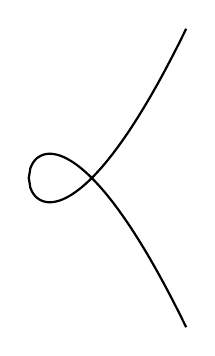
\begin{tikzpicture}[samples=300, scale=0.8]
            \draw[thick, domain=-1:1.5, samples=100] plot(\x,{sqrt(\x+1)*(abs(\x))});
            \draw[thick, domain=-1:1.5, samples=100] plot(\x,{-sqrt(\x+1)*(abs(\x))});
        \end{tikzpicture}
    \end{minipage}
    \begin{minipage}{.2\textwidth}
        \centering
        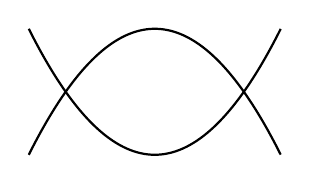
\begin{tikzpicture}[scale=0.8]
            \draw[thick, domain=-2:2, samples=100] plot(\x, {(1/2)*(\x)^2 - 1});
            \draw[thick, domain=-2:2, samples=100] plot(\x, {(-1/2)*(\x)^2 + 1});
        \end{tikzpicture}
    \end{minipage}
    \begin{minipage}{.2\textwidth}
        \centering
        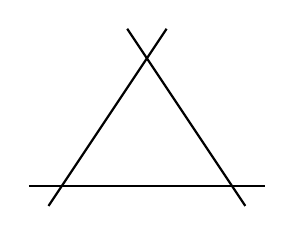
\begin{tikzpicture}[scale=0.25]
            \draw[thick] (-9,-1)--(-3,8);
            \draw[thick] (-10,0)--(2,0);
            \draw[thick] (1,-1)--(-5,8);
        \end{tikzpicture}
    \end{minipage}
    \begin{minipage}{.2\textwidth}
        \centering
        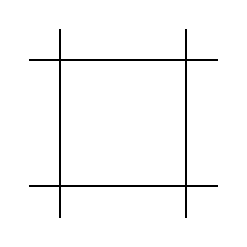
\begin{tikzpicture}[scale=0.4]
            % fiber
            \draw[thick] (-3, -2)--(3, -2);
            \draw[thick] (-3, 2)--(3, 2);
            \draw[thick] (-2, -3)--(-2, 3);
            \draw[thick] (2, -3)--(2, 3);
        \end{tikzpicture}
    \end{minipage}
    \caption{Kodaira fibers of type $\rom{1}_1$, $\rom{1}_2$, $\rom{1}_3$, and $\rom{1}_4$, respectively.}
    \label{fig:kodaira-fibers}
\end{figure}

If $F$ is reducible, then every irreducible component $G$ (with the reduced subscheme structure) of $F$ is a $(-2)$-curve on the surface $S$.
The line bundle $\cO_G(a)$ on $G \cong \bP^1$ with degree $a \in \bZ$, viewed as an object of the category $D^b(F)$, induces a spherical object $i_*\cO_G(a) \in D^b(S)$, and gives the half-spherical twist $H_{\cO_G(a)} \in \Auteq D^b(S)$ (Example \ref{ex:half-spherical-twist-from-kodaira-fiber}).
They satisfy the following relations in general.

\begin{proposition}[braid relations]\label{prop:braid-relation}
    Let $G$ and $G'$ be irreducible components of a reducible fiber $F$.
    \begin{enumerate}
        \item If $G \cdot G' = 1$, then we have
              \begin{equation}
                  H_{\cO_G(a)} \circ H_{\cO_{G'}(a')} \circ H_{\cO_G(a)} \cong H_{\cO_{G'}(a')} \circ H_{\cO_G(a)} \circ H_{\cO_{G'}(a')}
              \end{equation}
              for any $a, a' \in \bZ$.
        \item If $G \cap G' = \emptyset$, then we have
              \begin{equation}
                  H_{\cO_G(a)} \circ H_{\cO_{G'}(a')} \cong H_{\cO_{G'}(a')} \circ H_{\cO_G(a)}.
              \end{equation}
              for any $a, a' \in \bZ$.
    \end{enumerate}
\end{proposition}
\begin{proof}
    There are corresponding braid relations for the spherical twists $T_{\cO_G(a)}$ and $T_{\cO_{G'}(a')}$ in $\Auteq D^b(S)$ \cite[Example 3.5]{MR1831820}.
    The ``restriction'' morphism $j^*$ from Proposition \ref{prop:restriction-to-fiber} or Definition \ref{def:half-spherical-twist} maps these relations to the ones in the statement.
\end{proof}

\begin{proposition}\label{prop:half-spherical-twist-and-line-bundle}
    Let $G$ be an irreducible component of a reducible fiber $F$.
    Then we have
    $H_{\cO_G(a-1)} \circ H_{\cO_G(a)} \cong (-) \otimes \cO_{S}(G)\lvert_{F}$.
\end{proposition}
\begin{proof}
    For a smooth surface $S$, a $(-2)$-curve $G \subset S$, and an integer $a \in \bZ$, we have a relation $T_{\cO_G(a-1)} \circ T_{\cO_G(a)} \cong (-) \otimes \cO_{S}(G)$ in $\Auteq D^b(S)$ (\cite[Lemma 4.15 (i)(2)]{MR2198807}).
    Then the proposition follows.
\end{proof}


\subsection{Homological mirror symmetry}
We will describe the half-spherical twists $H_{\cO_G(a)}$ in terms of homological mirror symmetry.
Let us denote the Kodaira fiber of type $\rom{1}_{n}$ by $F_n$ and the $n$-punctured $2$-torus by $T_n$.
They are known to form a mirror pair due to the result of Lekili and Polishchuk.
\begin{theorem}[\cite{MR3663596}]\label{thm:mirror-symmetry-for-F_n}
    There is a $\bC$-linear triangulated equivalence
    \begin{equation}
        D^b(F_n) \cong D^b(\cW(T_n))
    \end{equation}
    between the derived category of $F_n$ and the wrapped Fukaya category of $T_n$.
\end{theorem}
\begin{remark}
    For the other types of Kodaira fibers, their mirror partners (or even candidates of mirrors) are not known yet.
\end{remark}
This equivalence suggests that spherical objects and some autoequivalences of $D^b(F_n)$ correspond to closed curves and mapping classes of $T_n$, respectively.
For more detailed formulations of such correspondence, we refer to \cite{opper2023spherical}.
\begin{theorem}[{\cite[Theorem A, Proposition 7.13]{opper2023spherical}}]\label{thm:bijection-between-objects-and-curves}
    There exists a bijection between isomorphism classes of indecomposable objects of $D^b(F_n)$ up to shift, and homotopy classes of curves on $T_n$ equipped with indecomposable local systems.
    Moreover, under this bijection, spherical objects correspond to non-separating simple loops with one-dimensional local systems.
\end{theorem}
\begin{theorem}[{\cite[Proposition 3.10, Theorem 7.22]{opper2023spherical}}]\label{intersections_are_morphisms}
    Let $\cF$ and $\cG$ be indecomposable objects of $D^b(F_n)$ which correspond to $(\gamma_{\cF}, V_{\cF})$ and $(\gamma_{\cG}, V_{\cG})$ by Theorem \ref{thm:bijection-between-objects-and-curves}, respectively.
    Here $\gamma_{\cF}, \gamma_{\cG}$ are homotopy classes of curves on $T_n$ and $V_{\cF}, V_{\cG}$ are local systems on these curves.
    Suppose that either $\cF$ or $\cG$ is perfect and $\dim V_{\cF} = \dim V_{\cG} = 1$. Then $\gamma_{\cF}$ and $\gamma_{\cG}$ have precisely $\sum_{i}\dim\Ext^i(\cF, \cG)$ intersections.
\end{theorem}
\begin{theorem}[{\cite[Theorem D]{opper2023spherical}}]\label{thm:autoequivalence-of-I_n-curve}
    Assume $n \geq 2$.
    The group of autoequivalences $\Auteq{D^b(F_n)}$ fits into the short exact sequence
    \begin{equation}
        1 \to \Aut^0(F_n) \times \Pic^0(F_n) \times \bZ[1] \to \Auteq{D^b(F_n)} \xrightarrow{\Upsilon} \MCG(T_n) \to 1,
    \end{equation}
    where $\Pic^0(F_n)$ denotes the group of line bundles with multi-degree zero, and $\Aut^0(F_n) \cong (\bC^\times)^n$ denotes the group of autoequivalences fixing the irreducible components of $F_n$.
\end{theorem}
\begin{theorem}[{\cite[Corollary 7.37]{opper2023spherical}}]\label{thm:definition-of-upsilon}
    The morphism $\Upsilon$ in Theorem \ref{thm:autoequivalence-of-I_n-curve} respects the correspondence in Theorem \ref{thm:bijection-between-objects-and-curves} in the following sense:
    For an element $\Phi \in \Auteq{D^b(F_n)}$, the mapping class $\Upsilon(\Phi)$ acts on the set of homotopy classes of curves on $T_n$ by $\gamma_{\cF} \mapsto \gamma_{\Phi(\cF)}$, where $\gamma_{\cF}$ is the curve on $T_n$ corresponding to an indecomposable object $\cF \in D^b(F_n)$.
\end{theorem}
\begin{theorem}[{\cite[Theorem 5.9]{opper2023spherical}}]\label{thm:spherical-twist-and-dehn-twist}
    Let $\cE \in D^b(F_n)$ be a spherical object and $(\gamma_{\cE}, V_{\cE})$ be the corresponding loop and local system. Then the morphism $\Upsilon$ in Theorem \ref{thm:autoequivalence-of-I_n-curve} maps the twist functor $T_{\cE}$ to the Dehn twist $T_{\gamma_{\cE}}$ along $\gamma_{\cE}$.
\end{theorem}

From now on, we denote the curve corresponding to an indecomposable object $E \in D^b(F_n)$ by $\gamma_{\cE}$.


\begin{example}
    Figure \ref{fig:corresponding-curves-via-hms} shows some examples of Theorem \ref{thm:bijection-between-objects-and-curves}.
    The big rectangle illustrates the $n$-punctured torus $T_n$.
    The top and bottom edges (resp.~ the left and right edges) are identified and the white circles represent the punctures.

    Take an irreducible decomposition $F_n = G_1 \cup \cdots \cup G_n$ with cyclic order and pick a smooth point $x_i$ from each component $G_i$.
    The structure sheaves $\cO_{F_n}, \cO_{x_1}, \dots, \cO_{x_n}$ of $F_n$ and the points $x_i$ are spherical objects of $D^b(F_n)$.
    They correspond to non-separating simple loops $\gamma_{\cO_{F_n}}, \gamma_{\cO_{x_1}}, \dots, \gamma_{\cO_{x_n}}$ on $T_n$ which are shown in Figure \ref{fig:corresponding-curves-via-hms}.
    Additionally, every sheaf of the form $\cO_{G_i}(a)$ is an indecomposable object that is not perfect (and hence not spherical).
    The corresponding curves $\gamma_{\cO_{x_i}}(-1)$ are not loops but arcs connecting two punctures.
\end{example}

\begin{figure}[h]
    \centering
    \begin{displaymath}
        \begin{tikzpicture}[scale=1.2]
            % big square
            \draw[dashed] (0,0)--(11,0);
            \draw[dashed] (0,0)--(0,4);
            \draw[dashed] (0,4)--(11,4);
            \draw[dashed] (11,4)--(11,0);

            % horizontal lines
            \draw[thick] (0, 2)--(1, 2);
            \draw[thick] (1, 2)--(3, 2);
            \draw[thick] (3, 2)--(5, 2);
            \draw[thick] (9, 2)--(11, 2);

            \draw[thick] (0, 0.5)--(11, 0.5);

            % vertical lines
            \draw[thick] (2, 0)--(2, 4);
            \draw[thick] (4, 0)--(4, 4);
            \draw[thick] (10, 0)--(10, 4);

            % punctures
            \draw[dotted, thick] (5+1, 2)--(9-1, 2);
            \foreach \u in {1, 3, 5, 9}
                {
                    \filldraw[white] (\u, 2) circle (2pt);
                    \draw[black] (\u, 2) circle (2pt);
                }

            % notations
            \draw(0, 0.5) node[left]{$\gamma_{\cO_{F_n}}$};
            \draw(2, 4) node[above]{$\gamma_{\cO_{x_1}}$};
            \draw(4, 4) node[above]{$\gamma_{\cO_{x_2}}$};
            \draw(10, 4) node[above]{$\gamma_{\cO_{x_n}}$};

            \draw(2, 3) node[above left]{$\gamma_{\cO_{G_1}(-1)}$};
            \draw(1, 3) to[out=-90,in=135](1.5, 2);
            \draw(4, 3) node[above left]{$\gamma_{\cO_{G_2}(-1)}$};
            \draw(3, 3) to[out=-90,in=135](3.5, 2);

            \draw(11, 2) node[right]{$\gamma_{\cO_{G_n}(-1)}$};

        \end{tikzpicture}
    \end{displaymath}
    \caption{The curves $\gamma_{\cO_{F_n}}, \gamma_{\cO_{x_i}}$ and $\gamma_{\cO_{G_i}(-1)}$ on the $n$-punctured torus $T_n$.}
    \label{fig:corresponding-curves-via-hms}
\end{figure}

\begin{example}
    For an irreducible component $G \subset F_n$ and $a \in \bZ$, the curve $\gamma_{\cO_G(a)}$ corresponding to the sheaf $\cO_G(a) \in D^b(F_n)$ is shown in Figure \ref{geometric_picture_of_induced_autoequivalences_1} or \ref{geometric_picture_of_induced_autoequivalences_2}.
    It is an arc wrapping around the torus $|a + 1|$ times and its direction is determined by the sign of $a + 1$.
    When $a = -1$ we get the curve $\gamma_{\cO_G(-1)}$ which is already shown in Figure \ref{fig:corresponding-curves-via-hms}.
\end{example}

\begin{figure}[h]
    \centering
    \begin{displaymath}
        \begin{tikzpicture}
            % big square
            \draw[dashed] (0,0)--(11,0);
            \draw[dashed] (0,0)--(0,4);
            \draw[dashed] (0,4)--(11,4);
            \draw[dashed] (11,4)--(11,0);

            % curves
            \draw[thick] (2, 2)--(2.5, 0);
            \draw[thick] (2.5, 4)--(3.5, 0);
            \draw[thick] (3.5, 4)--(4.5, 0);

            \draw[dotted, thick] (4.5, 2)--(6, 2);

            \draw[thick] (6.5, 4)--(7, 2);


            % punctures
            \foreach \u in {2, 7}
                {
                    \filldraw[white] (\u, 2) circle (2pt);
                    \draw[black] (\u, 2) circle (2pt);
                }

            % notations
            \draw(2.5, 4) node[above]{$\gamma$};

            \draw[
                thick,
                decoration={
                        brace,
                        mirror,
                        raise=0.5cm
                    },
                decorate
            ] (2.5, 0) -- (7, 0);
            \draw(4.5, -1) node{$a+1$ times};

        \end{tikzpicture}
    \end{displaymath}
    \caption{The curve $\gamma = \gamma_{\cO_G(a)}$ for $a+1>0$.}
    \label{geometric_picture_of_induced_autoequivalences_1}
\end{figure}

\begin{figure}[h]
    \centering
    \begin{displaymath}
        \begin{tikzpicture}
            % big square
            \draw[dashed] (0,0)--(11,0);
            \draw[dashed] (0,0)--(0,4);
            \draw[dashed] (0,4)--(11,4);
            \draw[dashed] (11,4)--(11,0);

            % curves
            \draw[thick] (2, 2)--(2.5, 4);
            \draw[thick] (2.5, 0)--(3.5, 4);
            \draw[thick] (3.5, 0)--(4.5, 4);

            \draw[dotted, thick] (4.5, 2)--(6, 2);

            \draw[thick] (6.5, 0)--(7, 2);


            % punctures
            \foreach \u in {2, 7}
                {
                    \filldraw[white] (\u, 2) circle (2pt);
                    \draw[black] (\u, 2) circle (2pt);
                }

            % notations
            \draw(2.5, 4) node[above]{$\gamma$};

            \draw[
                thick,
                decoration={
                        brace,
                        mirror,
                        raise=0.5cm
                    },
                decorate
            ] (2.5, 0) -- (7, 0);
            \draw(4.5, -1) node{$-(a+1)$ times};

        \end{tikzpicture}
    \end{displaymath}
    \caption{The curve $\gamma = \gamma_{\cO_G(a)}$ for $a+1<0$.}
    \label{geometric_picture_of_induced_autoequivalences_2}
\end{figure}


Employing these pictures, we will give a topological description of the half-spherical twists $H_{\cO_G(a)}$.
To begin with, we prepare some computations of homological algebra.
\begin{lemma}
    Let $F$ be a reducible fiber of $\pi \colon S \to C$.
    For an irreducible component $G \subset F$ of $F$, we have the following.
    \begin{enumerate}
        \item $\Ext^*_S(\cO_G(-1), \cO_F) = 0$.
        \item $\Ext^*_S(\cO_G(-1), \cO_x) = 0$ for every point $x \in F \setminus G$.
        \item $\Ext^*_S(\cO_G(-1), \cO_x) = \bC\oplus\bC[-1]$ for every point $x \in G$.
    \end{enumerate}
\end{lemma}
\begin{proof}
    They are easily verified by using Serre duality and Riemann-Roch theorem.
\end{proof}
\begin{lemma}\label{lem:preparation}
    Let $F$ be a reducible fiber of $\pi \colon S \to C$ and $G \subset F$ be an irreducible component.
    Let $H = H_{\cO_G(-1)}$ be the half-spherical twist along $\cO_G(-1)$.
    Then we have the following.
    \begin{enumerate}
        \item $H(\cO_F) \cong \cO_F$.
        \item $H(\cO_x) \cong \cO_x$ for every point $x \in F \setminus G$.
        \item For every point $x \in G$, there is an exact triangle  \begin{equation}
                  \cO_G(-2)[1]\to H(\cO_x)\to \cO_G(-1) \xrightarrow{+1}
              \end{equation}
              in $D^b(F)$.
    \end{enumerate}
\end{lemma}
\begin{proof}
    From the previous lemma, we have $\cO_F \in \langle \cO_G(-1) \rangle^\perp \subset D^b(S)$ and hence $T_{\cO_G(-1)}(\cO_F) \cong \cO_x$ (see Corollary \ref{cor:orthogonal-to-spherical}).
    Combining $i_* \circ H \cong T_{\cO_G(-1)} \circ i_*$ (Corollary \ref{cor:compatibility-of-half-spherical-twists-and-spherical-twists}), there is an isomorphism $i_*H(\cO_F) \cong T_{\cO_G(-1)}(\cO_F) \cong \cO_F$ in $D^b(S)$.
    Taking into account that $i$ is a closed immersion, it implies that $H(\cO_F)$ is a coherent sheaf on $F$ and therefore $H(\cO_F) \cong \cO_F$ in $D^b(F)$.
    This proves (1).
    The proof of (2) is similar.

    For (3), it is enough to prove the isomorphism of cohomology sheaves
    \begin{equation}
        \cH^i(T_{\cO_G(-1)}(\cO_x)) \cong \begin{cases}
            \cO_G(-1) & i = 0,            \\
            \cO_G(-2) & i = -1,           \\
            0         & \text{otherwise},
        \end{cases}
    \end{equation}
    for $x \in G$.
    This follows from the long exact sequence associated with the exact triangle
    \begin{equation}
        \Ext^*_S(\cO_G(-1), \cO_x) \otimes_\bC \cO_G(-1)\to \cO_x \to T_{\cO_G(-1)}(\cO_x) \xrightarrow{+1}
    \end{equation}
    and the previous lemma.
\end{proof}

\begin{lemma}\label{lem:preparation-2}
    Let $F = F_n$ be a reducible fiber of type $\rom{1}_n$ for $n \geq 3$, $G \subset F$ be an irreducible component, and $x \in G$ be a point which is a smooth point of $F$.
    Let $H = H_{\cO_G(-1)}$ be the half-spherical twist along $\cO_G(-1)$.
    Then we have the following.
    \begin{enumerate}
        \item $\Ext^*_F(H(\cO_{x}), \cO_{y}) =
                  \begin{cases}
                      \bC \oplus \bC[-1] & y \in G \text{: a smooth point of }F,              \\
                      0                  & y \in F \setminus G  \text{: a smooth point of }F.
                  \end{cases}$
        \item $\Ext^*_F(H(\cO_{x}), \cO_F) = \bC[-1]$.
        \item Let $G' \subset F$ be an irreducible component. Then \begin{equation}
                  \Ext^*_F(H(\cO_{x}), \cO_{G'}(-1)) = \begin{cases}
                      \bC     & G=G',                  \\
                      \bC[-1] & G\cdot G'=1,           \\
                      0       & G \cap G' = \emptyset.
                  \end{cases}
              \end{equation}
        \item $\Ext^*_F(H(\cO_{x}), \cO_{G}) = \bC^2 \oplus \bC[-1]$.
    \end{enumerate}
\end{lemma}
\begin{proof}
    They follow from the exact triangle in Lemma \ref{lem:preparation} (3) and the long exact sequences of $\Ext^*_F(-, \cO_{x}(-1))$, $\Ext^*_F(-, \cO_{F}(-1))$, $\Ext^*_F(-, \cO_{G'}(-1))$, and $\Ext^*_F(-, \cO_{G})$.
\end{proof}


\begin{theorem}\label{thm:half-spherical-twist-and-half-twist}
    Let $F = F_n$ be a reducible fiber of type $\rom{1}_n$ for $n \geq 3$.
    Let $G \subset F_n$ be an irreducible component, $a \in \bZ$ be an integer, and $H_{\cO_{G}(a)} \in \Auteq D^b(F_n)$ be the half-spherical twist along the sheaf $\cO_{G}(a)$.
    Then $H_{\cO_{G}(a)}$ is mapped to the half twist $h_{\gamma_{\cO_{G}(a)}}$ along the arc $\gamma_{\cO_{G}(a)}$ on $T_n$ by the morphism $\Upsilon$ in Theorem \ref{thm:definition-of-upsilon}:
    \begin{equation}
        \Upsilon \colon \Auteq D^b(F_n) \to \MCG(T_n), \quad H_{\cO_{G}(a)} \mapsto h_{\gamma_{\cO_{G}(a)}}.
    \end{equation}
\end{theorem}
\begin{proof}
    First, we prove the statement in the case $a = -1$.
    Let us denote the half-spherical twist along the sheaf $\cO_{G}(-1)$ by $H$ and the half twist along the curve $\gamma_{\cO_{G}(-1)}$ by $h$.
    Our goal is $\Upsilon(H) = h$.
    By Dehn--Nielsen--Baer theorem \ref{thm:Dehn--Nielsen--Baer},
    it is enough to show that $\Upsilon(H)$ and $h$ induce the same action on $\pi_1(T_n)$.
    Moreover, we only need to examine the finite number of curves $\gamma_{\cO_{F_n}}, \gamma_{\cO_{x_1}}, \dots, \gamma_{\cO_{x_n}}$ of which homotopy classes generate $\pi_1(T_n)$ (see Figure \ref{fig:corresponding-curves-via-hms}).
    We may assume $G = G_1$ and $x_1 \in G_1$ without loss of generality.
    Then both $\Upsilon(H)$ and $h$ fix $\gamma_{\cO_{F_n}}, \gamma_{\cO_{x_2}}, \dots, \gamma_{\cO_{x_n}}$ by Proposition \ref{prop:empty-intersection} and
    definition of half twists.
    It remains to show that $\gamma = \Upsilon(H)(\gamma_{\cO_{x_1}})$ and $\gamma' = h(\gamma_{\cO_{x_1}})$ are homotopic.
    Note that $\gamma$ is (homotopic to) the curve corresponding to the object $H(\cO_{x_1})$ by Theorem \ref{thm:definition-of-upsilon} and a simple non-separating loop as $H(\cO_{x_1})$ is spherical.
    To attack this problem, we will mimic the proof of \cite[Corollary 7.27]{opper2023spherical}.
    We only consider the case $n \geq 3$.
    The case $n = 2$ can be treated similarly.
    There are identities
    \begin{align}
         & \Ext^*_{F_n}(H(\cO_{x_1}), \cO_{x_i}) = 0 \quad (i \neq 1),                \\
         & \Ext^*_{F_n}(H(\cO_{x_1}), \cO_{F_n}) = \bC[-1],                           \\
         & \Ext^*_{F_n}(H(\cO_{x_1}), \cO_{G_i}(-1)) = \begin{cases}
                                                           \bC     & i = 1,               \\
                                                           \bC[-1] & i = 2 \text{ or } n, \\
                                                           0       & \text{otherwise},
                                                       \end{cases} \\
         & \Ext^*_{F_n}(H(\cO_{x_1}), \cO_{x_1}) = \bC \oplus \bC[-1],                \\
         & \Ext^*_{F_n}(H(\cO_{x}), \cO_{G}) = \bC^2 \oplus \bC[-1]
    \end{align}
    by Lemma \ref{lem:preparation-2}, which implies, by Theorem \ref{intersections_are_morphisms},
    that the curve $\gamma = \gamma_{H(\cO_{x_1})}$
    \begin{enumerate}
        \item is disjoint from $\gamma_{\cO_{x_2}}, \dots, \gamma_{\cO{x_n}}$,
        \item intersects
              $\gamma_{O_{F_n}}$, $\gamma_{\cO_{G_1}(-1)}$,
              $\gamma_{\cO_{G_2}(-1)}, \gamma_{\cO_{G_n}(-1)}$ exactly once,
        \item intersects $\gamma_{\cO_{x_1}}$ exactly twice, and
        \item intersects $\gamma_{\cO_{G}}$ exactly three times.
    \end{enumerate}
    The first three data of intersections, combined with the fact that $\gamma$ is a simple non-separating loop, determine that the curve $\gamma$ is homotopic to either $h(\gamma_{\cO_{x_1}})$ or $h^{-1}(\gamma_{\cO_{x_1}})$, as depicted in Figure \ref{candidates_for_gamma}.
    The last condition (4) distinguishes these two as in Figure \ref{candidates_for_gamma} and we conclude that $\gamma = h(\gamma_{\cO_{x_1}})$ (up to homotopy).

    For general $a \in \bZ$, we employ Proposition \ref{prop:half-spherical-twist-and-line-bundle} and similar relations for half twists to use induction on $a$.
    Let us denote the spherical twist $T_{\cO_{x_i}} = (-)\otimes \cO(x_i)$ by $T_i$ and the Dehn twist along $\gamma_{\cO_{x_i}}$ by $t_i$.
    They are related by the identities $\Upsilon(T_i) = t_i$.
    We also denote $H_{\cO_{G_i}(a)}$ by $H_{i, a}$ and the half twist along $\gamma_{\cO_{G_i}(a)}$ by $h_{i, a}$.
    The Dehn twists and the half twists are known to satisfy the relations
    \begin{align}
        t_i h_{i, a} t_i^{-1}          & = h_{i, a+1},            \\
        h_{i, a} t_i h_{i, a} t_i^{-1} & = t_{i-1}t_i^{-2}t_{i+1}
    \end{align}
    for $i \in \bZ/n\bZ$ and $a \in \bZ$.
    The first relation follows from the definition of half twists and the second one is found in the proof of \cite[Corollary 2.11]{MR1805936}, for instance.
    Combining these relations, we have relations
    \begin{equation}\label{eq:relation-between-half-twists-and-dehn-twists}
        h_{i, a}h_{i, a+1} = t_{i-1}t_i^{-2}t_{i+1}
    \end{equation}
    in $\MCG(T_n)$ for all $i$ and $a$.
    On the other hand, by Proposition \ref{prop:half-spherical-twist-and-line-bundle}, we have
    \begin{equation}
        H_{i, a}\circ H_{i, a+1} = (-)\otimes \cO_S(G_i)\lvert_{F_n}
    \end{equation}
    in $\Auteq D^b(F_n)$.
    The morphism $\Upsilon$ maps the right hand side to $t_{i-1}t_i^{-2}t_{i+1}$ by the following observations:
    \begin{enumerate}
        \item The line bundles $\cO_S(G_i)\lvert_{F_n}$ and $\cO_{F_n}(x_{i-1}-2x_{i}+x_{i+1})$ have the same multi-degree.
        \item The group $\Pic^0(F_n)$ of multi-degree zero line bundles is contained in $\Ker \Upsilon$ (Theorem \ref{thm:autoequivalence-of-I_n-curve}).
        \item $(-) \otimes \cO_{F_n}(x_i) \cong T_i$ (Example \ref{ex:spherical-objects}).
        \item $\Upsilon(T_i) = t_i$ (Theorem \ref{thm:spherical-twist-and-dehn-twist}).
    \end{enumerate}
    Therefore we have relations
    \begin{equation}\label{eq:relation-between-half-spherical-twists-and-spherical-twists}
        \Upsilon(H_{i, a})\Upsilon(H_{i, a+1}) = t_{i-1}t_i^{-2}t_{i+1}
    \end{equation}
    in $\MCG(T_n)$.
    Comparing \eqref{eq:relation-between-half-twists-and-dehn-twists} and \eqref{eq:relation-between-half-spherical-twists-and-spherical-twists} and using the $a = -1$ case, the (forward and backward) induction on $a$ provides the desired identities $\Upsilon(H_{i, a}) = h_{i, a}$ for all $i$ and $a$.
\end{proof}





\begin{figure}[h]
    \centering
    \begin{displaymath}
        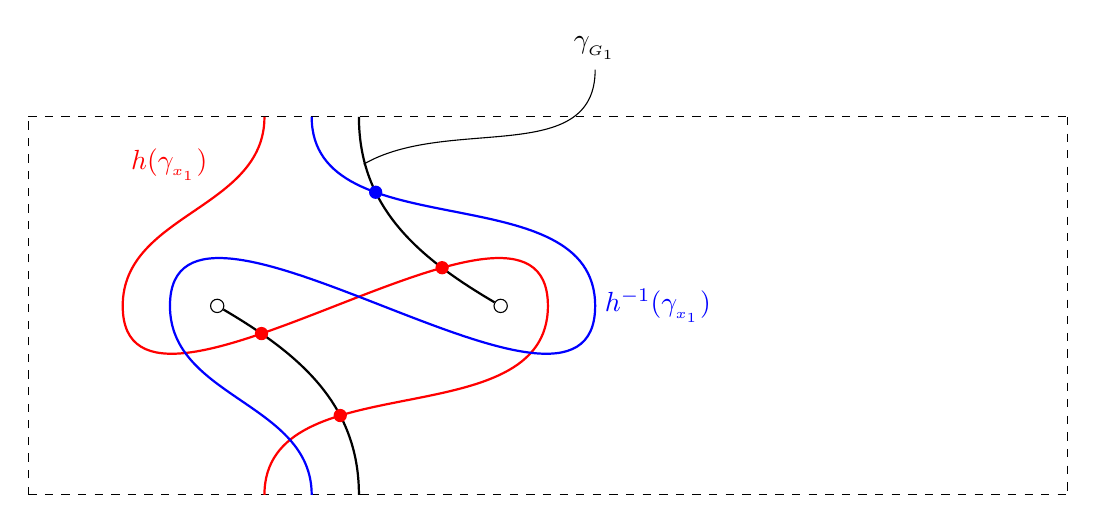
\begin{tikzpicture}[scale=1.2]
            % big square
            \draw[dashed] (0,0)--(11,0);
            \draw[dashed] (0,0)--(0,4);
            \draw[dashed] (0,4)--(11,4);
            \draw[dashed] (11,4)--(11,0);

            % curves
            \draw[thick, name path=black_1](3.5, 4) to[out=-90,in=150](5, 2);
            \draw[thick, name path=black_2](2, 2) to[out=-30,in=90](3.5, 0);

            \draw[thick, color=red](2.5, 4) to[out=-90,in=90](1, 2);
            \draw[thick, name path=red_2, color=red](1, 2) to[out=-90,in=90](5.5, 2);
            \draw[thick, name path=red_3, color=red](5.5, 2) to[out=-90,in=90](2.5, 0);

            \draw[thick, name path=blue_1, color=blue](3, 4) to[out=-90,in=90](6, 2);
            \draw[thick, color=blue](6, 2) to[out=-90,in=90](1.5, 2);
            \draw[thick, color=blue](1.5, 2) to[out=-90,in=90](3, 0);

            % punctures
            \foreach \u in {2, 5}
                {
                    \filldraw[white] (\u, 2) circle (2pt);
                    \draw[black] (\u, 2) circle (2pt);
                }

            % intersections
            \fill [name intersections={of=red_2 and black_1}, color=red]
            (intersection-1) circle (2pt) node [above right]{};
            \fill [name intersections={of=red_2 and black_2}, color=red]
            (intersection-1) circle (2pt) node [above right]{};
            \fill [name intersections={of=red_3 and black_2}, color=red]
            (intersection-1) circle (2pt) node [above right]{};

            \fill [name intersections={of=blue_1 and black_1}, color=blue]
            (intersection-1) circle (2pt) node [above right]{};

            % notations
            \draw[](2, 3.5) node[left, color=red]{$h(\gamma_{\cO_{x_1}})$};
            \draw[](6, 2) node[right, color=blue]{$h^{-1}(\gamma_{\cO_{x_1}})$};

            \draw(6, 4.5) node[above]{$\gamma_{\cO_{G_1}}$};
            \draw(6, 4.5) to[out=-90,in=30](3.55, 3.5);
        \end{tikzpicture}
    \end{displaymath}
    \caption{The two possible candidates for $\gamma$.} \label{candidates_for_gamma}
\end{figure}


\subsection{Autoequivalences of elliptic surfaces}
In this subsection, we give a refinement of Uehara's result Theorem \ref{thm:autoequivalence-of-elliptic-surface} by using the half-spherical twists.
Following \cite{MR3568337} we define a subgroup $B \subset \Auteq D^b(S)$ by
\begin{equation}
    B = \langle T_{\cO_G(a)} \mid G \subset S \text{ is an irreducible component of reducible fiber, } a \in \bZ\rangle.
\end{equation}


\begin{remark}\label{rem:alternative-description-of-minus-two-curves}
    If we assume that $S$ is projective and its Kodaira dimension $\kappa(S)$ is non-zero, the group $B$ coincides with the one in Theorem \ref{thm:autoequivalence-of-elliptic-surface}
    \begin{equation}
        B = \langle T_{\cO_G(a)} \mid G \subset S \text{ is a $(-2)$-curve, } a \in \bZ\rangle
    \end{equation}
    as mentioned in \cite[Section 3]{MR3568337}.
\end{remark}
By Proposition \ref{prop:twist-functor-is-in-FM}, the group $B$ can be viewed as a subgroup of $\FM_T(S)$ and we have a natural ``restriction'' morphism
\begin{equation}
    \res_F \colon B \hookrightarrow \FM_T(S) \to \FM_{\bC}(F) \hookrightarrow \Auteq D^b(F), \quad T_{\cO_G(a)} \mapsto H_{\cO_G(a)} \text{ if } G \subset F.
\end{equation}
Note that the restriction $\res_F(T_{\cO_G(a)})$ is trivial unless $F$ is the fiber containing $G$.
In order to capture the whole information of the group $B$, we need to consider the restriction morphisms $\res_F$ for all the reducible fibers $F$ at the same time.
Let $\res = \prod_{F \colon \text{reducible fiber}} \res_F$ be the product of these restriction morphisms.
\begin{proposition}\label{prop:kernel-of-res}
    We have an exact sequence
    \begin{equation}
        1 \to \langle (-) \otimes \cO_S(F) \mid F \text{: reducible fiber }\rangle \to B \xrightarrow{\res} \prod_{F \colon \text{reducible fiber}} \Auteq D^b(F).
    \end{equation}
\end{proposition}
\begin{proof}
    First of all, every equivalence $\Phi \in B$ satisfies $\Phi(\cO_x) \cong \cO_x$ for every point $x \in S \setminus \bigcup_{F \colon \text{reducible fiber}}F$ by Corollary \ref{cor:orthogonal-to-spherical}.
    Let $F \subset S$ be a reducible fiber and $i_F \colon F \hookrightarrow S$ be the inclusion.
    If $\Phi \in \Ker(\res_F)$, then $\res_F(\Phi)$ satisfies the condition $\res_F(\Phi)(\cO_x) \cong \cO_x$ for every point $x \in F$ and we also have
    \begin{equation}
        \Phi(\cO_x) \cong (i_{F*} \circ \res_F(\Phi))(\cO_x) \cong i_{F*}(\cO_x) = \cO_x
    \end{equation}
    in $D^b(S)$.
    Combining these observations, we obtain $\Phi(\cO_x) \cong \cO_x$ for every $\Phi \in \Ker(\res) = \bigcap_{F \colon \text{reducible fiber}} \Ker(\res_F)$ and every point $x \in S$.
    This implies the inclusion $\Ker(\res) \subset \Pic(S)$ by Lemma \ref{lem:criterion-to-be-standard-functor} and hence $\Ker(\res) = B \cap \Ker \left(\Pic(S) \to \prod_{F \colon \text{reducible fiber}} \Pic(F)\right)$.

    We prove the identity
    \begin{equation}\label{eq:kernel-of-res}
        B \cap \Ker \left(\Pic(S) \to \prod_{F \colon \text{reducible fiber}} \Pic(F)\right) = \langle (-) \otimes \cO_S(F) \mid F \text{: reducible fiber }\rangle.
    \end{equation}
    The inclusion $(\text{LHS}) \supset (\text{RHS})$ follows from \cite[Lemma 4.15 (i)(2)]{MR2198807}.
    To prove the other inclusion, let $L \in \Pic(S)$ be a line bundle such that $(-) \otimes L$ is an element of the right-hand side.
    The proof of \cite[Lemma 4.18 (i)]{MR2198807} shows that $L$ lies in the group
    \begin{equation}
        \Gamma = \langle \cO_S(G) \mid G \text{ is an irreducible component of a reducible fiber }\rangle \subset \Pic(S).
    \end{equation}
    Let $G_{jk}$ be the $k$-th irreducible component of the $j$-th reducible fiber and define
    \begin{equation}
        \Gamma_j = \langle \cO_S(G_{jk}) \mid k  \rangle \subset \Gamma.
    \end{equation}
    The group $\Gamma$ splits into the direct sum $\Gamma = \bigoplus_{j} \Gamma_j$ and it induces the decomposition $L = \bigotimes_{j} L_j$, where $L_j \in \Gamma_j$.
    The condition $L \in \Ker(\Pic(S) \to \prod_{F \colon \text{reducible fiber}} \Pic(F))$ implies that $L_j \lvert_{G_{jk}} = 0$ for every $j$ and $k$.
    Consequently, the intersection number $L_j \cdot G_{jk}$ on $S$ must be zero.

    Here we consider the $\bQ$-vector space $V_j$ generated by the irreducible components $\{G_{jk}\}_k$ of the $j$-th reducible fiber $F = F^{(j)}$ in the ($\bQ$-coefficient) N\'{e}ron--Severi group $\NS(S) \otimes \bQ$, together with the intersection form.
    It is well known that the set $\{G_{jk}\}$ gives a basis for $V_j$ and the intersection form on $V_j$ has exactly one-dimensional kernel, which is spanned by the class of $F^{(j)}$ (see \cite{MR1078016}, for example).
    The conditions $L_j \cdot G_{jk} = 0$ and $L_j \in \Gamma_j$ give the equations $L_j \cdot L_j = 0$ of intersection numbers.
    These observations imply that $L_j$ is a multiple of $F^{(j)}$ in $\NS(S) \otimes \bQ$.
    Then we have $L_j \in \langle \cO_S(F^{(j)}) \rangle \subset \Pic(S)$ and hence $L \in (\text{RHS of \eqref{eq:kernel-of-res}})$, because the map
    \begin{equation}
        \Gamma_j \hookrightarrow \Pic(S) \twoheadrightarrow \NS(S) \hookrightarrow \NS(S) \otimes \bQ
    \end{equation}
    is injective.
\end{proof}




\begin{theorem}\label{thm:description-of-B}
    Suppose that all the reducible fibers of the elliptic surface $\pi \colon S \to C$ are of type $\rom{1}_n$ (for some $n \geq 2$, depending on each fiber).
    Let $F^{(1)}, \dots, F^{(r)}$ be the reducible fibers and $n_j$ be the number of irreducible components of $F^{(j)}$.
    Then the following statements hold.
    \begin{enumerate}
        \item The exact sequence in Proposition \ref{prop:kernel-of-res} together with the morphism $\Upsilon$ in Theorem \ref{thm:spherical-twist-and-dehn-twist} induces the exact sequence
              \begin{equation}
                  1 \to \langle (-)\otimes \cO_S(F^{(j)}) \mid 1 \leq j \leq r \rangle \to B \xrightarrow{\psi} \prod_{j = 1}^r \MCG(T_{n_j}).
              \end{equation}
        \item Let $p_j \colon \prod_{j=1}^r \MCG(T_{n_j}) \to \MCG(T_{n_j})$ be the projection onto the $j$-th component. Then the image $\Image(\psi)$ is the product of its projections onto the individual components $\Image(\psi) = \prod_{j = 1}^r \Image(p_j \circ \psi)$.
        \item The set of half twists along the curves $\gamma_{\cO_{G_1}(-1)}, \dots, \gamma_{\cO_{G_{n_j}}(-1)}, \gamma_{\cO_{G_1}}, \dots, \gamma_{\cO_{G_{n_j}}}$ on $T_{n_j}$ generates the subgroup $\Image(p_j \circ \psi) \subset \MCG(T_{n_j})$ (see Figure \ref{fig:generators-for-image-of-B}).
        \item If $\kappa(S) \neq 0$, then the group $B$ coincides with the group
              \begin{equation}
                  \langle T_{\cO_G(a)} \mid G \subset S \text{ is a $(-2)$ curve, } a \in \bZ\rangle,
              \end{equation}
              which was originally denoted by $B$ in \cite{MR3568337}.
    \end{enumerate}
\end{theorem}

\begin{figure}[h]
    \centering
    \begin{displaymath}
        \begin{tikzpicture}[scale=1.2]
            % big square
            \draw[dashed] (0,0)--(10,0);
            \draw[dashed] (0,0)--(0,4);
            \draw[dashed] (0,4)--(10,4);
            \draw[dashed] (10,4)--(10,0);

            % horizontal lines
            \draw[thick] (0, 2)--(1, 2);
            \draw[thick] (1, 2)--(3, 2);
            \draw[thick] (3, 2)--(5, 2);
            \draw[thick] (5, 2)--(6, 2);
            \draw[thick] (8, 2)--(9, 2);
            \draw[thick] (9, 2)--(10, 2);


            % vertical lines
            \draw[thick] (0, 4)--(1, 2);
            \draw[thick] (1, 2)--(2, 0);
            \draw[thick] (2, 4)--(4, 0);
            \draw[thick] (4, 4)--(5, 2);
            \draw[thick] (5, 2)--(5.5, 1);
            \draw[thick] (8.5, 3)--(9, 2);
            \draw[thick] (9, 2)--(10, 0);

            % punctures
            \draw[dotted, thick] (5+1.5, 2)--(9-1.5, 2);
            \foreach \u in {1, 3, 5, 9}
                {
                    \filldraw[white] (\u, 2) circle (2pt);
                    \draw[black] (\u, 2) circle (2pt);
                }

            % notations
            \draw(2, 0) node[below]{$\gamma_{\cO_{G_1}}$};
            \draw(4, 0) node[below]{$\gamma_{\cO_{G_2}}$};
            \draw(10, 0) node[below]{$\gamma_{\cO_{G_{n_j}}}$};

            \draw(2, 3) node[above left]{$\gamma_{\cO_{G_1}(-1)}$};
            \draw(1, 3) to[out=-90,in=135](1.5, 2);
            \draw(4, 3) node[above left]{$\gamma_{\cO_{G_2}(-1)}$};
            \draw(3, 3) to[out=-90,in=135](3.5, 2);

            \draw(10, 2) node[right]{$\gamma_{\cO_{G_{n_j}}(-1)}$};

        \end{tikzpicture}
    \end{displaymath}
    \caption{The simple arcs such that the half twists along them generate $\Image(B \xrightarrow{p_j \circ \psi} \MCG(T_{n_j}))$.} \label{fig:generators-for-image-of-B}
\end{figure}
\begin{proof}
    The morphism $\psi$ in (1) is defined by the composition
    \begin{equation}
        \psi = \prod_{j=1}^r \Upsilon_j \circ \res_j \colon B \to \Auteq D^b(F^{(j)}) \to \MCG(T_{n_j}),
    \end{equation}
    where $\Upsilon_j$ is the morphism $\Upsilon$ in Theorem \ref{thm:spherical-twist-and-dehn-twist} for the reducible fiber $F^{(j)}$.
    We need to prove that the morphism
    \begin{equation}
        \Image\left(\res_j = \res_{F^{(j)}} \colon B \to \Auteq D^b(F^{(j)})\right) \xrightarrow{\Upsilon} \MCG(T_{n_j})
    \end{equation}
    is injective for each $j$.
    Suppose that $\Phi \in B$ satisfies
    \begin{equation}
        \res_j(\Phi) = \varphi_*(L \otimes (-))[n] \in \Ker(\Upsilon) = \Aut^0(F^{(j)})\times \Pic^0(F^{(j)}) \times \bZ[1]
    \end{equation}
    for some $\varphi \in \Aut^0(F^{(j)})$, $L \in \Pic(F^{(j)})$, and $n \in \bZ$.
    We want to prove $\res_j(\Phi) = \id$.
    Note that we may assume $\Phi$ is a composition of the functors
    \begin{equation}
        \{T_{\cO_{G}(a)} \mid G \subset F^{(j)} \colon \text{irreducible component}, a \in \bZ\}
    \end{equation}
    because the contribution from the other reducible fibers does not change the image $\res_j(\Phi)$.
    Then we have
    \begin{equation}\label{eq:condition_for_Phi}
        \Phi(\cO_x) \cong \begin{cases}
            \cO_x               & x \in S \setminus F^{(j)}, \\
            \cO_{\varphi(x)}[n] & x \in F^{(j)}.
        \end{cases}
    \end{equation}
    Now Lemma \ref{lem:criterion-to-be-standard-functor} can be applied to $\Phi$ so that $\Phi$ is of the form $\widetilde{\varphi}_*(- \otimes \widetilde{L})$ for some $\widetilde{\varphi}\in \Aut{S}$ and $\widetilde{L} \in \Pic{S}$, and $n = 0$.
    The automorphism $\widetilde{\varphi}$ must be the identity by \eqref{eq:condition_for_Phi} and the continuity.
    Therefore we have $\varphi = \widetilde{\varphi}\lvert_{F^{(j)}} = \id_{F^{(j)}}$ and $L = \widetilde{L}\lvert_{F^{(j)}} \in \Pic^0(F^{(j)})$.
    Since $\Phi = (-) \otimes \widetilde{L}$ is in $B \cap \Pic(S)$, the line bundle $\widetilde{L}$ is an element of the group $\Gamma \subset \Pic(S)$ appeared in the proof of the previous proposition.
    The condition $\widetilde{L}\lvert_{F^{(j)}} \in \Pic^0(F^{(j)})$ means that the restriction $\widetilde{L} \lvert_{G_{jk}}$ to an irreducible component $G_{jk} \subset F^{(j)}$ is trivial.
    Again by the same argument in the proof of the previous proposition, the line bundle $L = \widetilde{L}\lvert_{F^{(j)}}$ turns out to be trivial.
    This implies $\res_j(\Phi) = \id$.

    The statement (2) follows from the fact that for any generator $T_{\cO_G(a)} \in B$ there exists a reducible fiber $F$ such that $G \subset F$.

    The image $\Image(p_j \circ \psi \colon B \to \MCG(T_{n_j}))$ does not change when we restrict the domain to the subgroup $B_j = \langle T_{\cO_G(a)} \mid G \subset F^{(j)}, a \in \bZ \rangle \subset B$.
    To show (3), it is enough to prove the group $B_j$ is generated by $T_{\cO_{G_1}}, \dots, T_{\cO_{G_{n_j}}}, T_{\cO_{G_1}(-1)}, \dots, T_{\cO_{G_{n_j}}(-1)}$.
    This is an immediate consequence of the relation $T_{\cO_G(a)} \circ T_{\cO_G(a+1)} = (-)\otimes \cO_S(G)$ for a surface $S$ and a $(-2)$-curve $G$ \cite[Lemma 4.15 (i)]{MR2198807}.

    The last statement (4) is just a rephrasing of Remark \ref{rem:alternative-description-of-minus-two-curves}.
\end{proof}


\begin{remark}\label{rm:psi-is-not-surjective}
    The morphism $\psi \colon B \to \prod_{j=1}^r \MCG(T_{n_j})$ is not surjective.
    For example, the Dehn twist along the curve $\gamma_{\cO_{x_1}} \subset T_{n_j}$ (see Figure \ref{fig:generators-for-image-of-B}),
    or equivalently,
    the twist functor $T_{\cO_{x_1}} = (-)\otimes \cO_{F^{(j)}}(x_1) \in \Auteq{D^b(F^{(j)})}$ cannot be obtained from the elements of $B$.
    We can prove this as follows.
    Assume $j = 1$ for simplicity and set $n = n_1$, $F = F^{(1)} = G_1 \cup \cdots \cup G_n$.
    Every element $(-) \otimes L \in \Image(B \to \Auteq D^b(F)) \cap \Pic F$ comes from a line bundle in $\langle \cO_S(G_k) \mid k = 1, \dots, n\rangle \in \Pic S$ by a similar argument to the proof of Theorem \ref{prop:kernel-of-res}.
    Then the sum of all components of the multi-degree vector of $L$ must be zero, and thus $L \ncong \cO_{F}(x_1)$.
\end{remark}

% \begin{remark}
%     Let $F_n$ be the Kodaira fiber of type $\rom{1}_n$ and $\PMCG(T_n) \subset \MCG(T_n)$ be the \emph{pure mapping class group} consisting of the mapping classes which fix the individual punctures.
%     Motivated by homological mirror symmetry (HMS) for $F_n$ and $T_n$, Sibilla \cite{MR3182005} explicitly constructed an action on $D^b(F_n)$ of the \emph{graded} pure mapping class group $\widetilde{\PMCG}(T_n)$, which is a central extension of $\PMCG(T_n)$ by $\bZ$,
%     and conjectured that this action is faithful.
%     By using recent developments in HMS such as \cite{MR3735868, MR3830878}, one can extend the action to the whole graded mapping class group $\widetilde{\MCG(T_n)}$ and prove its faithfulness as stated in \cite{opper2023spherical}.

%     On the other hand, the mapping class group $\MCG(T_n)$ is generated by the set of half twists along certain arcs and the subgroup $\PMCG(T_n)$ \cite{MR1805936}.
%     Our results will give an alternative way to construct the action of $\widetilde{\MCG}(T_n)$ on $D^b(F_n)$ avoiding HMS, as Sibilla did.
%     It is an interesting problem to consider the same story for the other types of Kodaira fibers, for which HMS is not established yet.
% \end{remark}


% \begin{remark}
%     For an irreducible component $G$ of a reducible fiber $F_n$ of type $\rom{1}_n$ and $a \in \bZ$, there is an isomorphism
%     \begin{equation}
%         \Ext_{F_n}^*(\cO_G(a), \cO_G(a)) \cong \bC[x, y]/(xy).
%     \end{equation}
%     of graded $\bC$-algebras, where $\deg(x) = \deg(y) = 2$.
%     We can observe that the latter one coincides with $H_{S^1}^*(S^2, \bC)$, the \emph{$S^1$-equivariant cohomology ring of the sphere $S^2$}.
%     In this sense, the sheaf $\cO_G(a)$ can be regarded as a ``$S^1$-equivariant version'' of spherical objects.
%     This observation might be related to ``$S^1$-equivariant'' mirror symmetry, which is explained in \cite{lekili2023equivariant} for example.
% \end{remark}

\begin{remark}
    Let
    $
        \overline{S} \coloneqq \Spec \bC[x,y,z]/(x y - z^{n+1})
        \subset \Spec \bC[x,y,z] \cong \bA^3
    $
    be an affine surface with an $A_n$-singularity at the origin
    and
    $
        \overline{f} \colon \overline{S} \to \Spec \bC[z]
    $
    be the projection to the $z$-axis.
    Let further
    $
        \pi \colon S \to \overline{S}
    $
    be the minimal resolution
    and
    $
        f \coloneqq \overline{f} \circ \pi
    $
    be the composite morphism.
    The fiber
    $
        F
        \coloneqq f^{-1}(0)
    $
    is the union
    of the exceptional locus
    $
        E \coloneqq \bigcup_{i=1}^n G_i
    $
    of the resolution $\pi$
    and two copies of the affine line.
    Note that if $n=1$ the same situation can also be obtained from Example \ref{example_from_Atiyah_flop} by cutting with the hyperplane $\{z=w\}$.
    which are strict transforms of the
    coordinate lines
    $
        \Spec \bC[x,y,z]/(xy, z)
        \cong \Spec \bC[x] \cup \Spec \bC[y].
    $
    There is a homomorphism
    \begin{align}
        \rho \colon B_n^{(1)} \to \Auteq(D^b(S))
    \end{align}
    from the \emph{affine braid group}
    $
        B_n^{(1)}
    $
    generated by $\sigma_i$ for $i=0,\ldots,n$
    with relations
    \begin{align}
        \sigma_i \sigma_{i+1} \sigma_i & = \sigma_{i+1} \sigma_i \sigma_{i+1}, &  & i = 0, \ldots, n \quad(\sigma_{n+1} \coloneqq \sigma_0), \\
        \sigma_i \sigma_j              & = \sigma_j \sigma_i,                  &  & |i-j|>2,
    \end{align}
    sending $\sigma_0$ to $T_{\omega_E}$
    and $\sigma_i$ to
    $
        T_{\cO_{G_i}(-1)}
    $
    for $i=1, \ldots, n$.
    Proposition \ref{prop:restriction-to-fiber}. gives
    a homomorphism
    \begin{align}
        \res_F \colon \Image \rho \to \Auteq D^b(F).
    \end{align}
    One has an equivalence
    \begin{align} \label{eq:HMS}
        D^b(F) \simeq \cW(\Sigma_{0,n+3})
    \end{align}
    where $\cW(\Sigma_{0,n+3})$
    is the wrapped Fukaya category of a surface $\Sigma_{0,n+3}$
    of genus 0 with $n+3$ punctures
    equipped with a suitable grading
    \cite{MR3735868, MR3830878}.
    The composite $\res_F \circ \rho$
    together with the equivalence \eqref{eq:HMS}
    gives an affine braid group action
    on $\cW(\Sigma_{0,n+3})$,
    which factors the graded mapping class group
    of $\Sigma_{0,n+3}$
    just as in the case of Kodaira fibers discussed above.
    This implies the injectivity of $\rho$,
    which is one of the main results of
    \cite{MR2629510}.
\end{remark}


\printbibliography
\end{document}